\chapter{Veto efficiency studies for the 2024 WIMP search result}\label{chap:VetoEfficiency}
A WIMP scatter is expected to only deposit a small amount of energy (few~keV) within the LXe volume of the experiment in a single scatter. Neutrons produced through radioactive decays within detector materials mimics a WIMP interaction when they scatter off Xe atoms. Veto detectors surrounding the central LXe volume also permits assessment of the local radioactivity environment, and thus to infer additional information on the backgrounds in the WIMP search region. A WIMP discovery will require excellent understanding of all background sources, which is best done through the characterization of those backgrounds in situ. Efficiency of the veto systems in the detection of the radiation produced by the backgrounds should be maximised whilst minimizing the impact of the veto selection on detector livetime in turn maximising the detector livetime available for the detection of WIMPs. \autoref{sec:VetoEff/simulation_improvements} describes the series of improvements to the detector simulation which were made prior to the WS2024 science run which aided the understanding of the response from the veto detector systems. The refinement of the veto selection algorithm is discussed alongside the impact that the veto selection had on the WS2024 result from \autoref{sec:VetoEff/VetoSelectionOptimisation} onwards.

\section{Improved Outer Detector Simulations}\label{sec:VetoEff/simulation_improvements}
Prior to WS2024 result, there were a number of major differences between simulations and data in the Outer Detector (OD). As such, an effort was made to correct this through modifications to the geometry of the Outer Detector in simulations to better reflect what is observed in data.
\subsection{Modifications of the Outer Detector simulation geometry}\label{sec:VetoEff/GeometryEdits}
There was a distinct discrepancy in neutron capture timing following single scatters within the TPC, this was one of the metrics which was investigated to quantify difference between data and simulation.
The simulation was improved through the following changes:
\begin{enumerate}
	%\item Spacing was added between the acrylic tanks to account for the gaps between the tanks which were present due to minor geometric differences produces in the moulding of the vessels during manufacturing process.
	\item Water was added to the foam volume which is between the OCV and acrylic tanks. The foam was intended to displace water to reduce neutron capture time however the foam became saturated with water \footnote{Later long-term bench top studies found that samples of foam became saturated with water.}.
	\item The acrylic tanks were moved further away from the OCV in the simulation to reflect the actual position of the tanks in the Outer Detector, as installed.
\end{enumerate}
A series of simulations were produced varying both the amount of water saturation of foam displacer in 1\% steps and the position of the acrylic tanks from the OCV in 10~mm steps. The \textit{best} configuration of the simulation geometry changes was found to be 30~mm and 6\% through matching the capture time of neutrons following single scatters in the active LXe volume. Additional details on the discrepancies between simulations and data with respect to neutron capture timing is given in the subsequent subsection.
\begin{figure}[ht!]
	\centering
	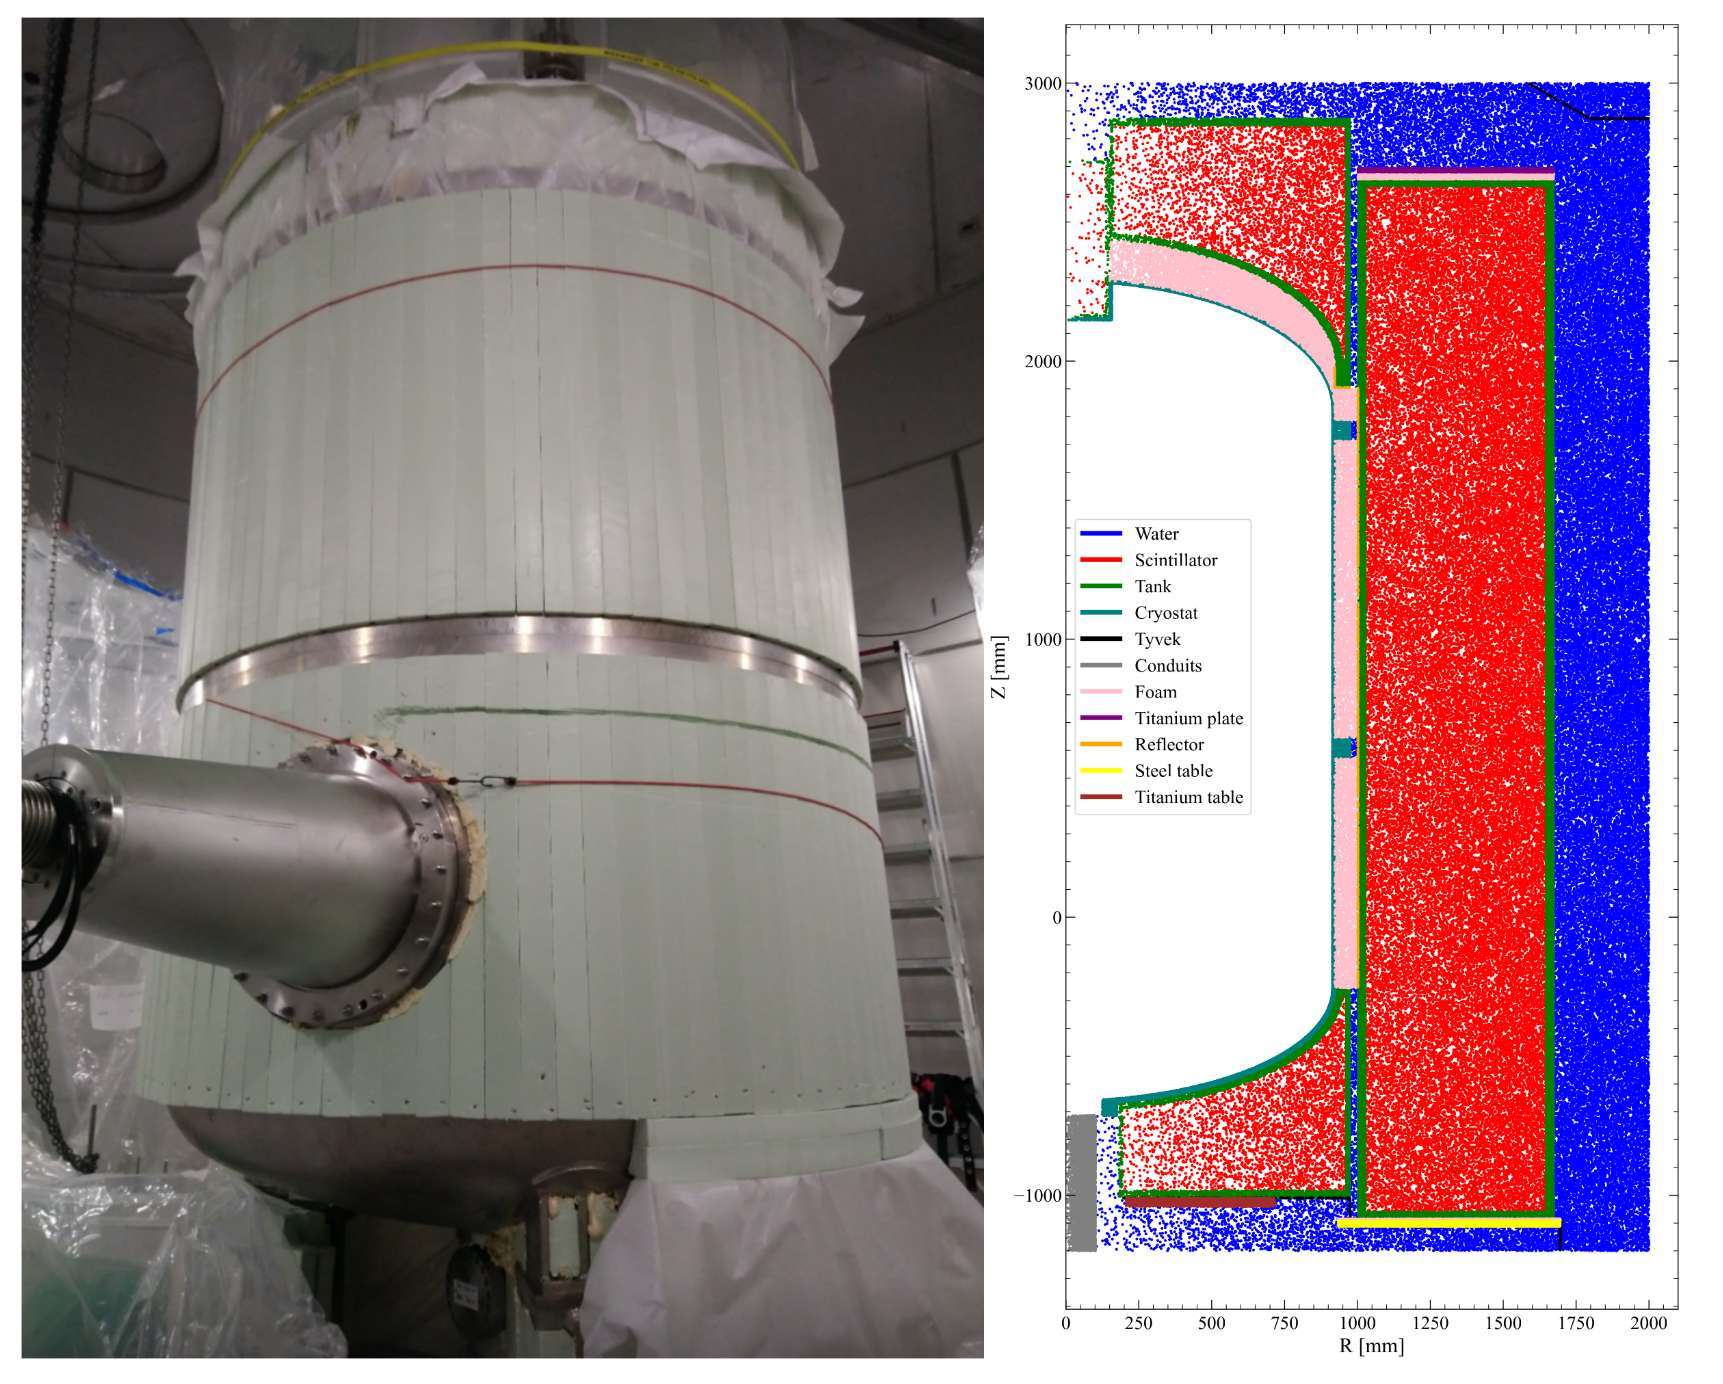
\includegraphics[width=0.9\textwidth]{figures/VetoEfficiency/FoamImgAndSimGeoTogether.png}
	\caption[An image of the foam displacer surrounding the OCS and final geometry in the simulation used for the WS2024 science run.]{Geometry in the simulation used for the WS2024 science run. \textbf{Left:} A photograph of the light green foam water displacer which resides between the acrylic tanks and the OCV. The water displacer was wrapped in a light reflector made from Tyvek. \textbf{Right:} A cross-section of the BACCARAT output. Geantinos were been passed through the simulation geometry, the $xyz$ position information and GEANT4 volumes were recorded to show the various volumes in the simulation.}
	\label{fig:VetoEff/od_geometry_for_sr3}
\end{figure}

\subsubsection{Neutron capture time}\label{sec:VetoEff/NCT}
Following the geometry changes discussed above, the neutron capture timing using AmLi was studied. Events which were classified as single scatters by LZap and passed the selection outlined in \autoref{tab:App_VetoEff/CoreCuts} in \autoref{app:VetoEff} were used for the study. OD pulses which exceeded a 200~keV (49~phd) threshold were used to optimise the geometry as this threshold is associated with proton recoil of neutrons of hydrogen in the OD medium.
All possible configurations of the geometry modifications were visually examined to determine which variation of simulation matched the data. An example of the comparison plot can be seen in \autoref{fig:VetoEff/NC_AmLi_50mm7}, the "baseline simulation" was the initially configuration of the geometry prior to this study. All plots were examined side by side in a large scale canvas configuration seen in Fig.\ref{fig:VetoEff/NC_Canvas0}, \ref{fig:VetoEff/NC_Canvas1}, \ref{fig:VetoEff/NC_Canvas2}, and \ref{fig:VetoEff/NC_Canvas3}. It was found that from this study that 30~mm~to~50~mm movement of the SATs alongside 5\%~to~7\% increase in the percentage of water in the foam provides the best agreement between data and simulation at a 200~keV threshold.
\begin{figure}[!ht]
	\centering
	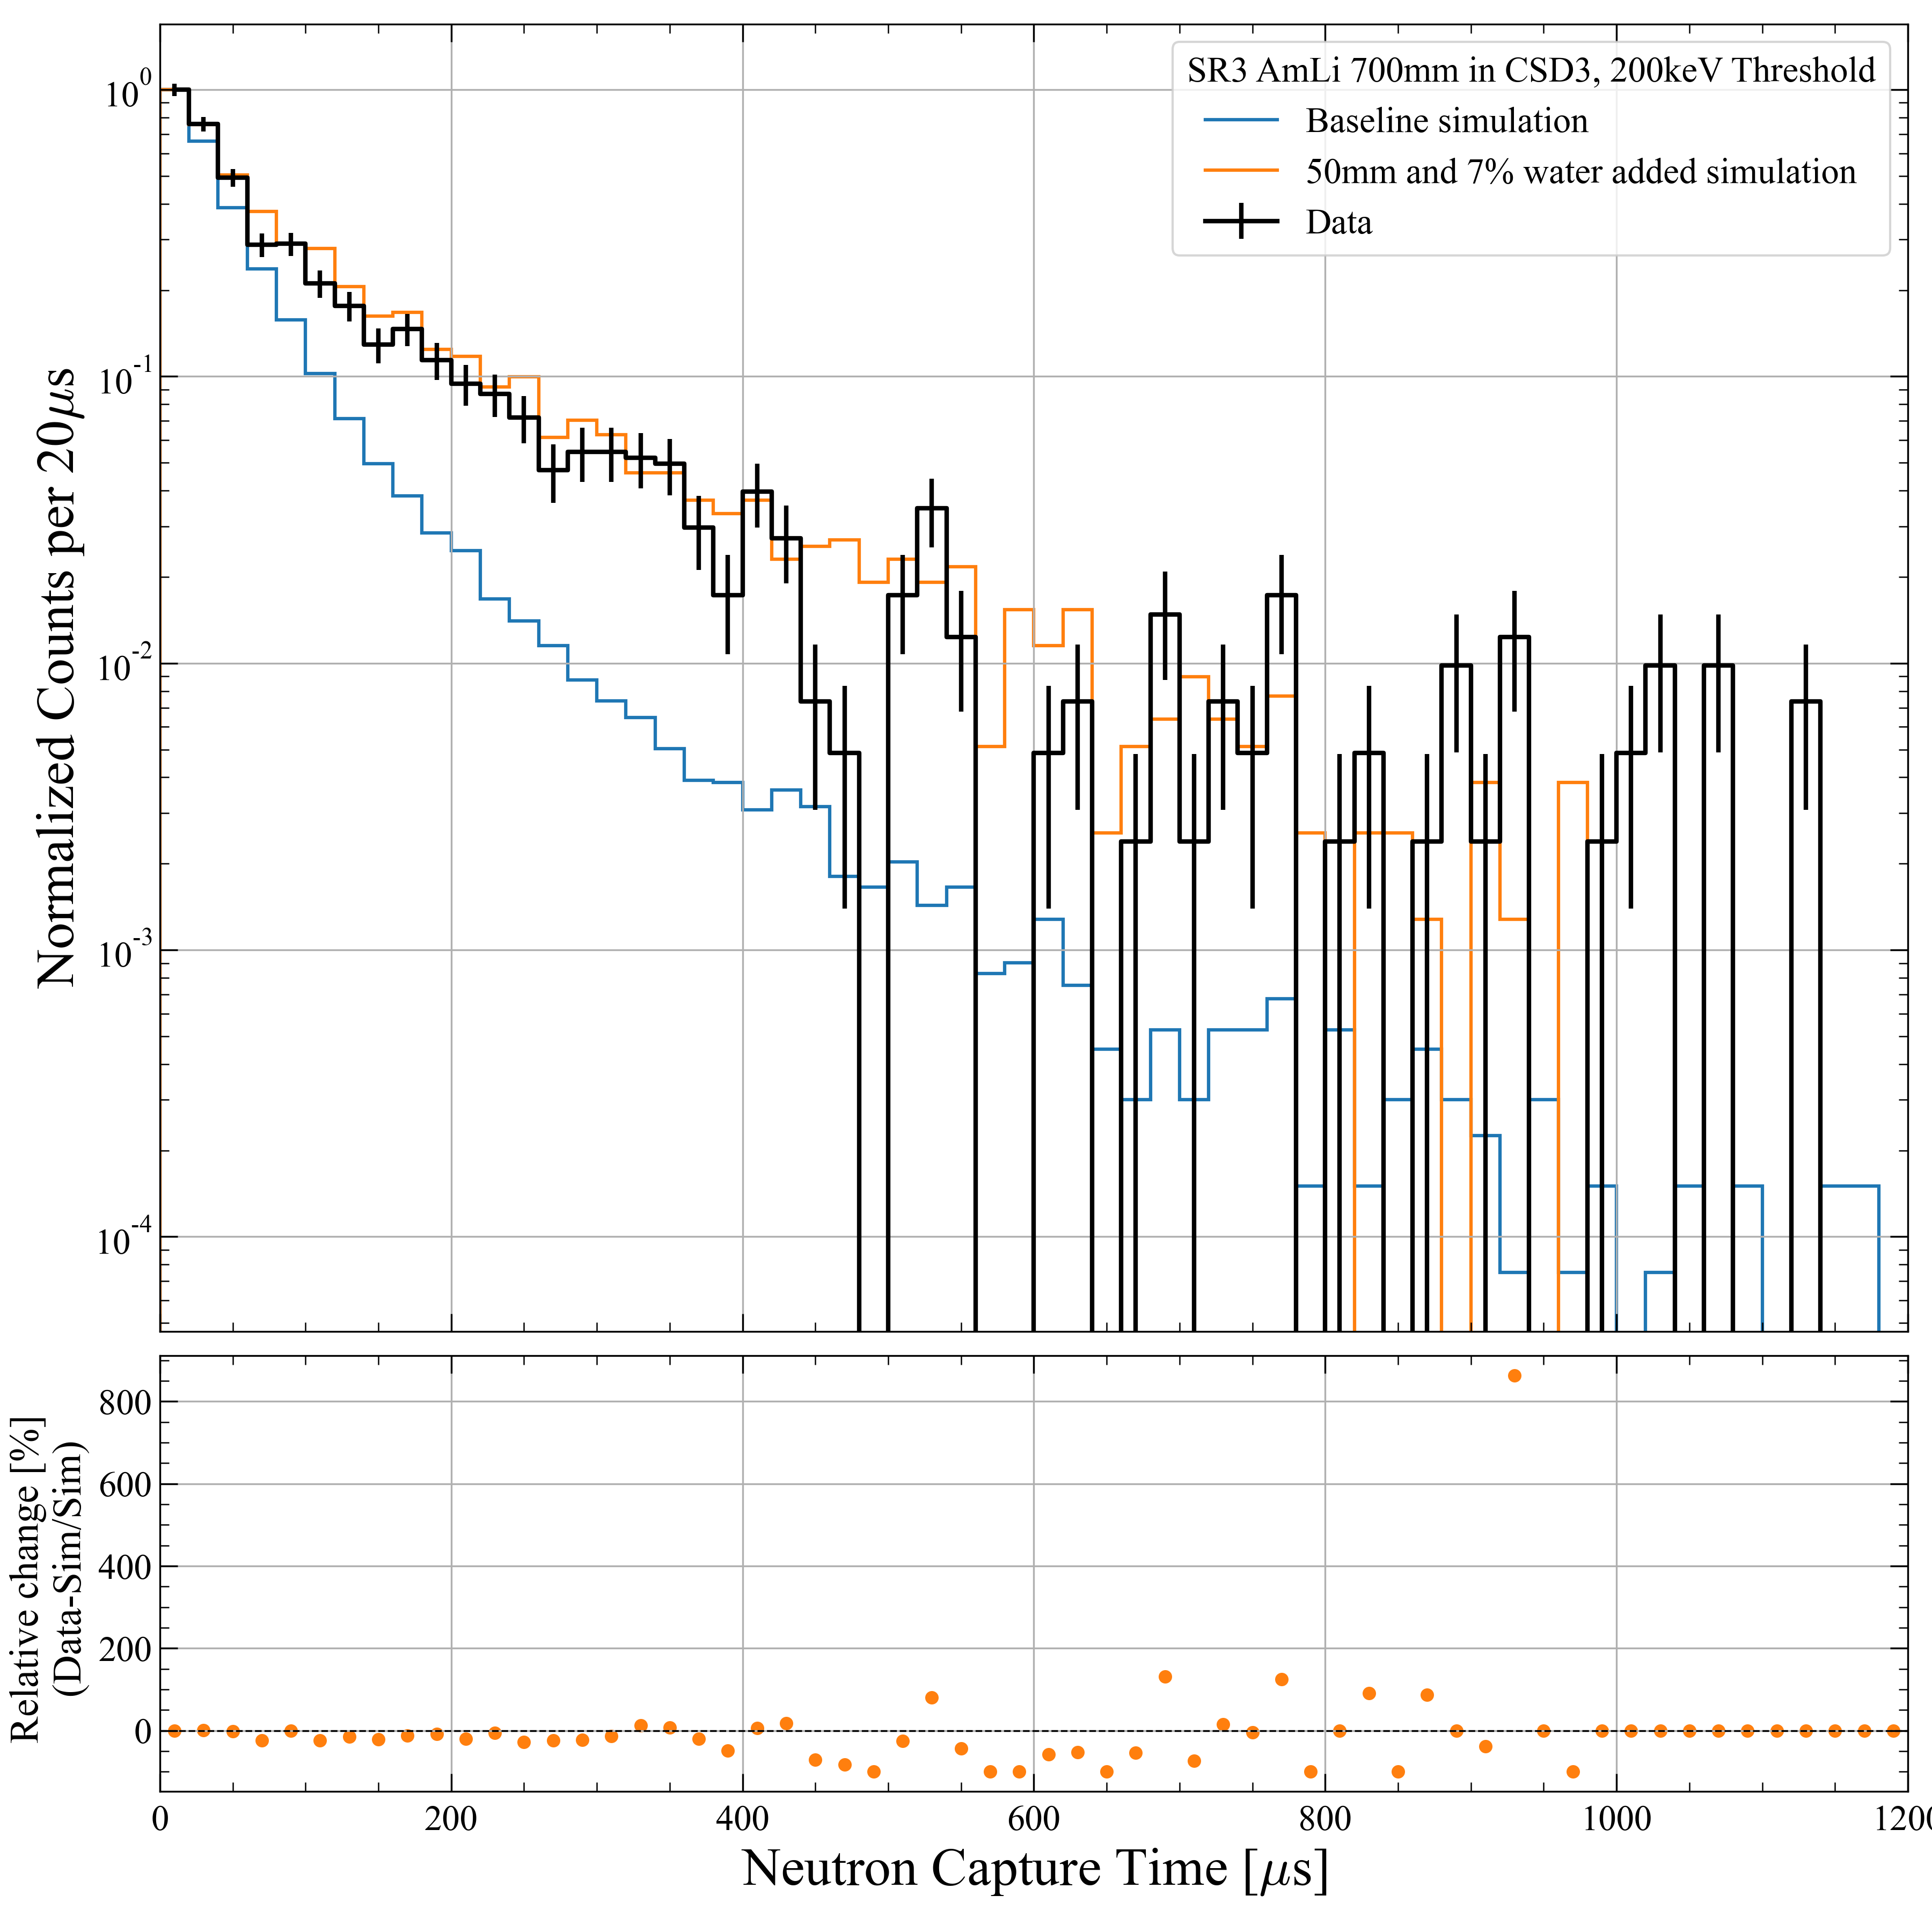
\includegraphics[width=0.7\linewidth]{figures/VetoEfficiency/movedSAT50mm_7percentWater_AmLi_CSD3_Z700mm_200keV_Ratio.png}
	\caption{An example of the plot used to compare neutron capture timing in data with the baseline simulation and the modified simulation. The relative change between data and simulation in each $20~\mu s$ bin was used to aid the visually examination across the $1200~\mu s$ window.}
	\label{fig:VetoEff/NC_AmLi_50mm7}
\end{figure}

\iffalse
\begin{sidewaysfigure}[ht!]
	\centering
	\includegraphics[width=\linewidth]{figures/VetoEfficiency/NCTiming_Canvas_700mm_AmLi.pdf}
	\caption{Large scale canvas of all possible simulation configurations. Each plot is similar in style to \autoref{fig:VetoEff/NC_AmLi_50mm7}. Here AmLi at 700mm above the cathode in CSD3 has been shown as an example.}
	\label{fig:VetoEff/NC_Canvas}
\end{sidewaysfigure}
\fi

\section{Veto selection optimisation}\label{sec:VetoEff/VetoSelectionOptimisation}
A description of how the veto selection for the WS2024 was optimised is presented in this section. The Skin and OD veto cuts used in the WS2024 science run were based on those developed for the WS2022 science run, described in \cite{LZCollaboration:2024lux} and are presented in \autoref{tab:VetoEff/sr3_veto_cuts}.
The veto selection relies on four separate selection criteria which each have their own intended purposes:
\begin{itemize}
	\item \textit{Skin-prompt} used for tagging $\gamma$-rays in the Skin detector
	\item \textit{OD-prompt} used for tagging $\gamma$-rays and neutron proton recoils in the OD
	\item \textit{Skin-delayed} used for tagging $\gamma$-rays from post-neutron capture de-excitation
	\item \textit{OD-delayed} used For tagging $\gamma$-rays from post-neutron capture de-excitation
\end{itemize}
The cuts used for the different veto criteria were selected at the same time as AmLi neutron tagging efficiency calculation, and were optimised to maximise the tagging efficiency whilst reducing deadtime. \textit{Pulse area} threshold, \textit{PMT coincidence} threshold and \textit{veto window length} are the three different variables which can be tuned for this optimisation. Events which were classified as single scatters by LZap and passed the selection outlined in \autoref{tab:VetoEff/amli_efficiency_cuts} were used for the study. The following subsections describe how each of the veto selection variables were tuned.

\begin{table}[!ht]
	\centering
	\caption{Outline of cuts applied to AmLi calibration data for determining the veto efficiency. All cuts are defined in \autoref{tab:App_VetoEff/CoreCuts}.}
	\label{tab:VetoEff/amli_efficiency_cuts}
    \scalebox{0.9}{
	\begin{tabular}{llll}
    \hline\hline
    \textbf{Livetime cuts}&\textbf{ Physics cuts}& \textbf{S2 cuts}& \textbf{S1 cuts}\\
    \hline
    Burst noise cut& Single scatter& S2 width vs drift time& S1 prominence cut\\
    Muon holdoff& S1 and S2 threshold & Narrow S2& Stinger event cut\\
    Sustained rate cut& Fiducial Volume& S2 rise time& S1 TBA vs drift time \\
    High S1 rate exclusion & & S2 early peak& S1 HSC cut\\
    Bad buffer cuts& & S2 XY quality& S1 shape\\
    Excess Area cut& & S2 TBA & S1 photon timing\\
    \hline\hline
	\end{tabular}}
\end{table}

\subsection{Veto window length}
The veto window length for the prompt windows were determined using AmLi and DD calibration data by measuring the time difference between the TPC single-scatter and OD and Skin pulses. The length of the prompt window is determined by width of the peak observed in the pulse timing distributions shown in both figures in \autoref{fig:VetoEff/veto_prompt_windows}. For the WS2024 selection, no change was made to the OD prompt veto window size, however the Skin prompt veto window was reduced by 500~ns as the number of the pulses observed outside of window $\pm250$~ns was considered negligible.
\begin{figure}[!ht]
	\centering
	\begin{subfigure}[b]{0.49\textwidth}
		\centering
		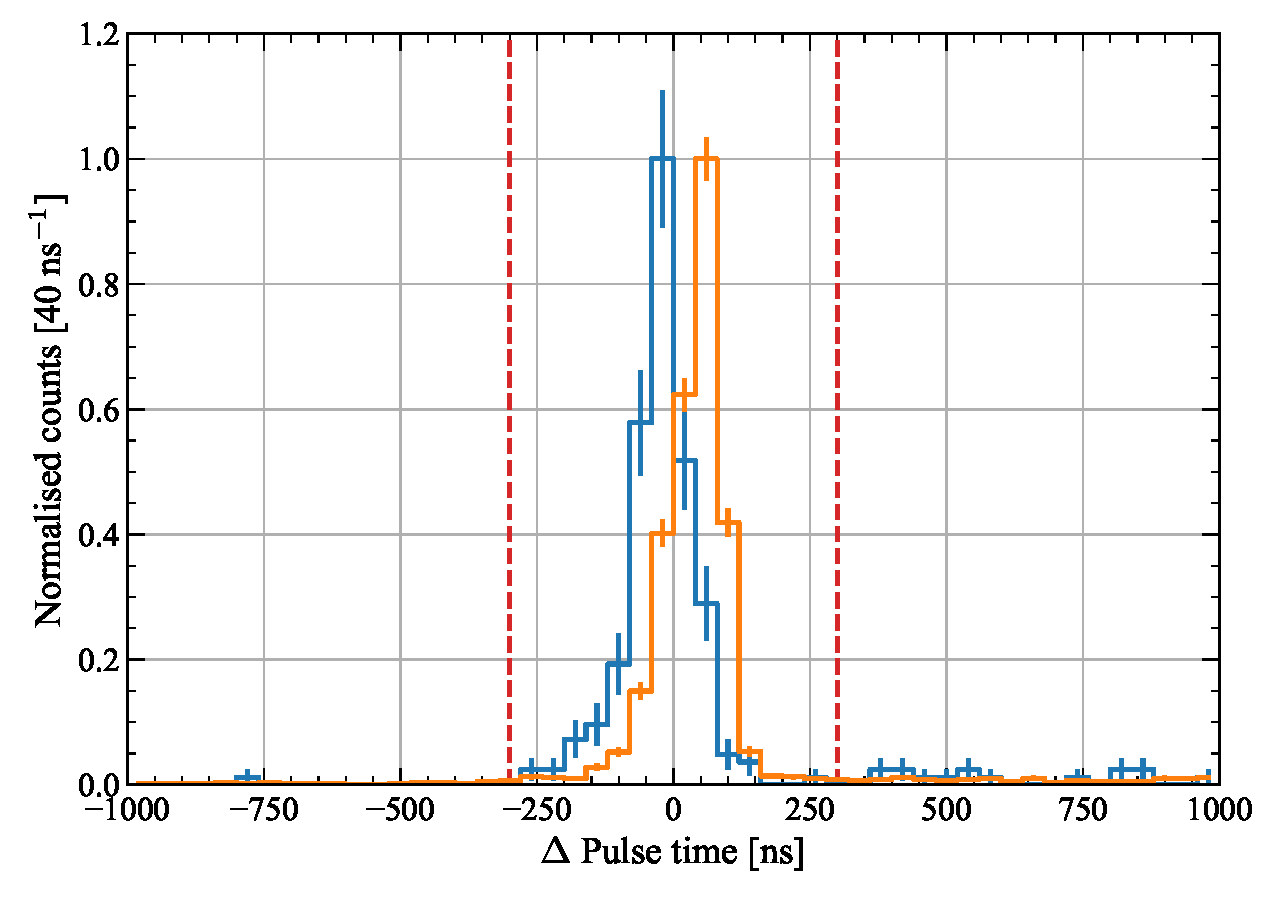
\includegraphics[width=\textwidth]{figures/VetoEfficiency/ODpromptWindowTiming.pdf}
		%\caption{Time difference (in ns) between TPC single-scatter and OD pulses using AmLi data.}
        \caption{}
		\label{fig:VetoEff/od_prompt_window}
	\end{subfigure}
	\hfill
	\begin{subfigure}[b]{0.49\textwidth}
		\centering
		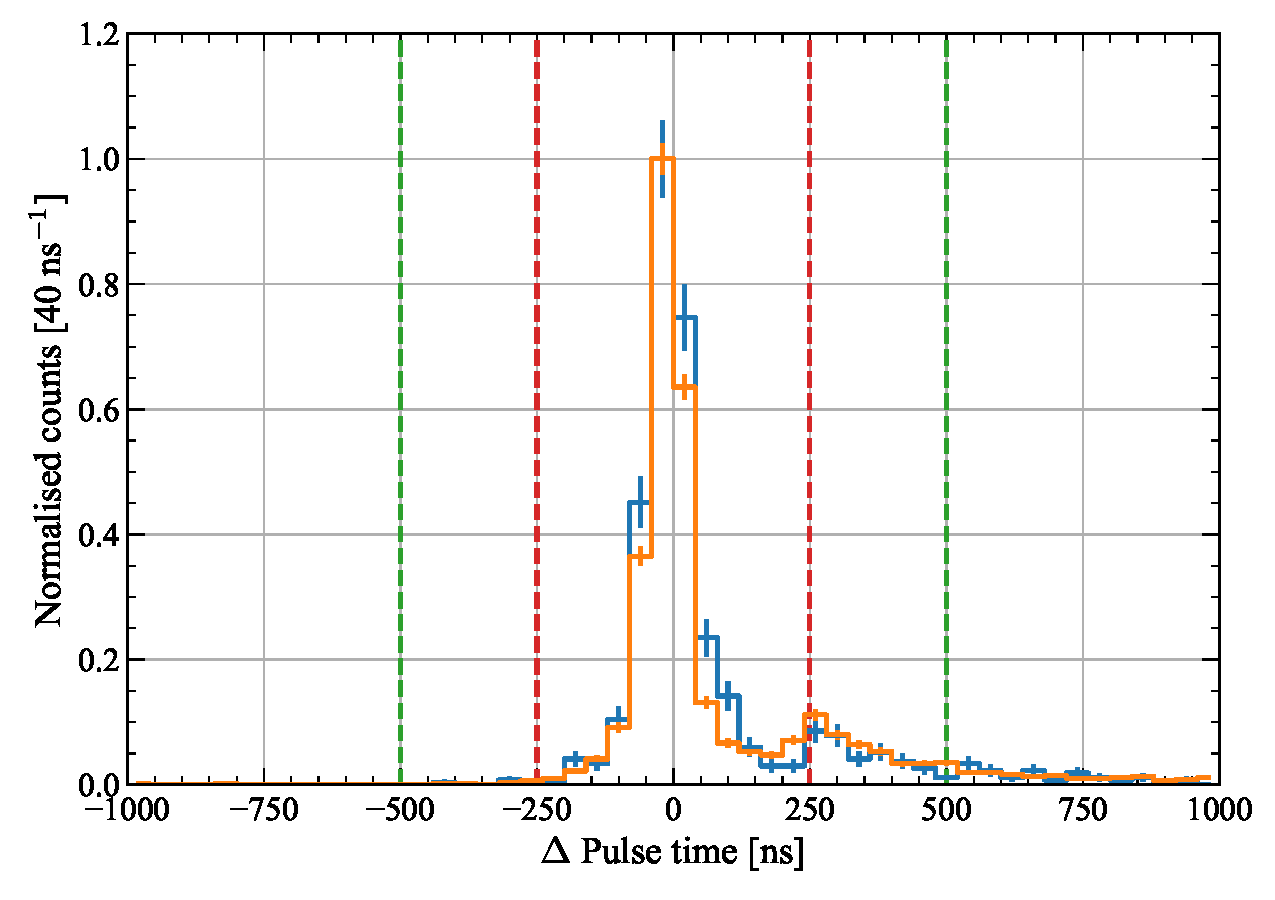
\includegraphics[width=\textwidth]{figures/VetoEfficiency/SkinpromptWindowTiming.pdf}
		%\caption{Time difference (in ns) between TPC single-scatter and OD pulses using DD data.}
		\caption{}
        \label{fig:VetoEff/skin_prompt_window}
	\end{subfigure}
	\caption{Prompt timing window for the OD (left) and Skin (right). %The time difference between TPC single scatter pulse and veto pulse was used to determine the optimal veto window size. 
    AmLi (blue) and DD (orange) calibration data was used to measure the time difference between the TPC single scatter pulse and veto pulse. 
    The vertical red lines indicate the boundary of the timing selection used for WS2024. There was no change in the size of the OD prompt veto window whereas the Skin prompt veto window was reduce by a total of 500~ns. The WS2022 veto window limits are shown in green.}
	\label{fig:VetoEff/veto_prompt_windows}
\end{figure}

The veto efficiency (defined in \ref{eqn:VetoEff/neutron_tagging_efficiency}) calculated using AmLi calibration data was used to determine the size of the delayed veto window for both the Skin and OD. The veto window length was reduced by a factor of two for both Skin and OD delayed windows as the slope of the efficiency curve began to plateau above 600~$\mu s$. An example of the veto efficiency plot used is shown in \autoref{fig:VetoEff/DelayedVetoWindow}.
\begin{figure}[!ht]
    \centering
    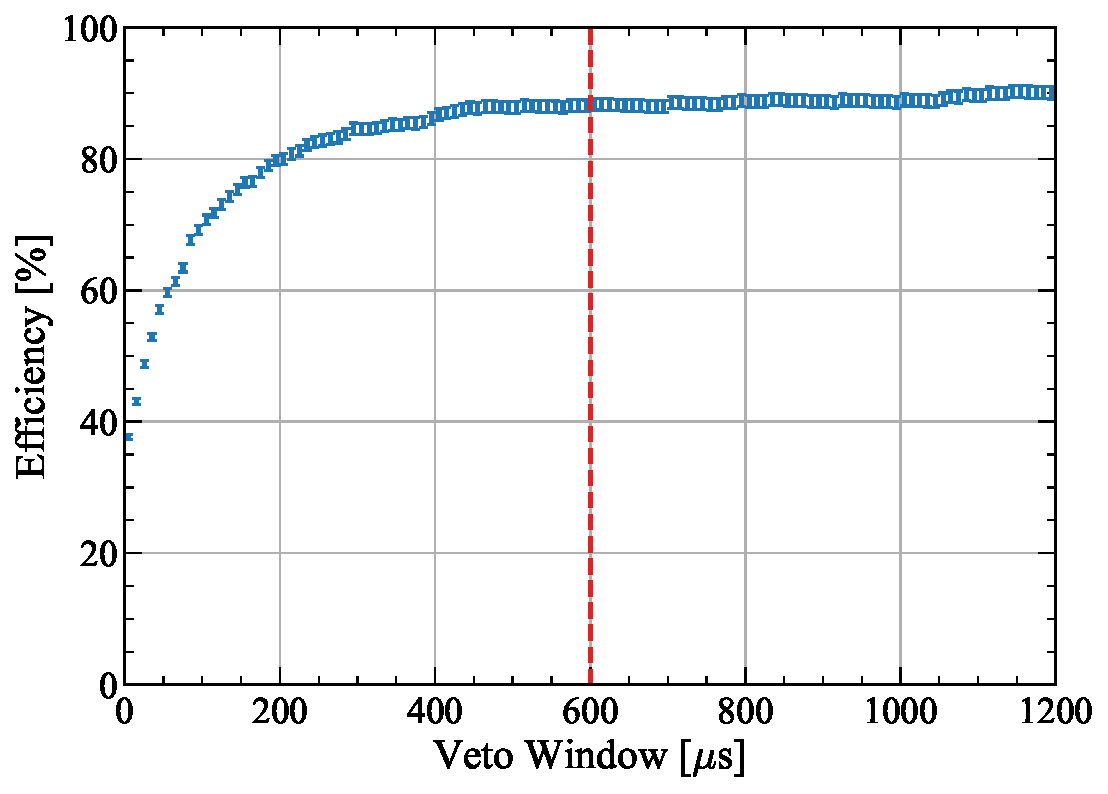
\includegraphics[width=0.5\linewidth]{figures/VetoEfficiency/DelayedVetoWindow.pdf}
    \caption{An example of a veto efficiency curve measured using AmLi calibration data. The vertical red line indicates the WS2024 upper bound of the delayed veto windows used for both the Skin and OD.}
    \label{fig:VetoEff/DelayedVetoWindow}
\end{figure}

The reduction in the veto window lengths has a positive impact on the dead time induced by the veto selection. Veto dead time is discussed in greater detail \autoref{sec:VetoEff/DeadtimeStability}.

\subsection{PMT Coincidence and pulse area threshold}
To optimize the pulse area and PMT coincidence thresholds the veto efficiency and deadtime was calculated for different integer step changes of both the pulse area and PMT coincidence for the respective veto windows. Heatmaps of efficiency and deadtime based on PMT coincidence and pulse area threshold were produced, an example of a heatmap is shown in \autoref{fig:VetoEff/od_prompt_veto_heatmap}. All heatmaps produced for the optimization study are shown in \autoref{app:VetoHeatMapsSec}.

\begin{sidewaysfigure}
	\centering
	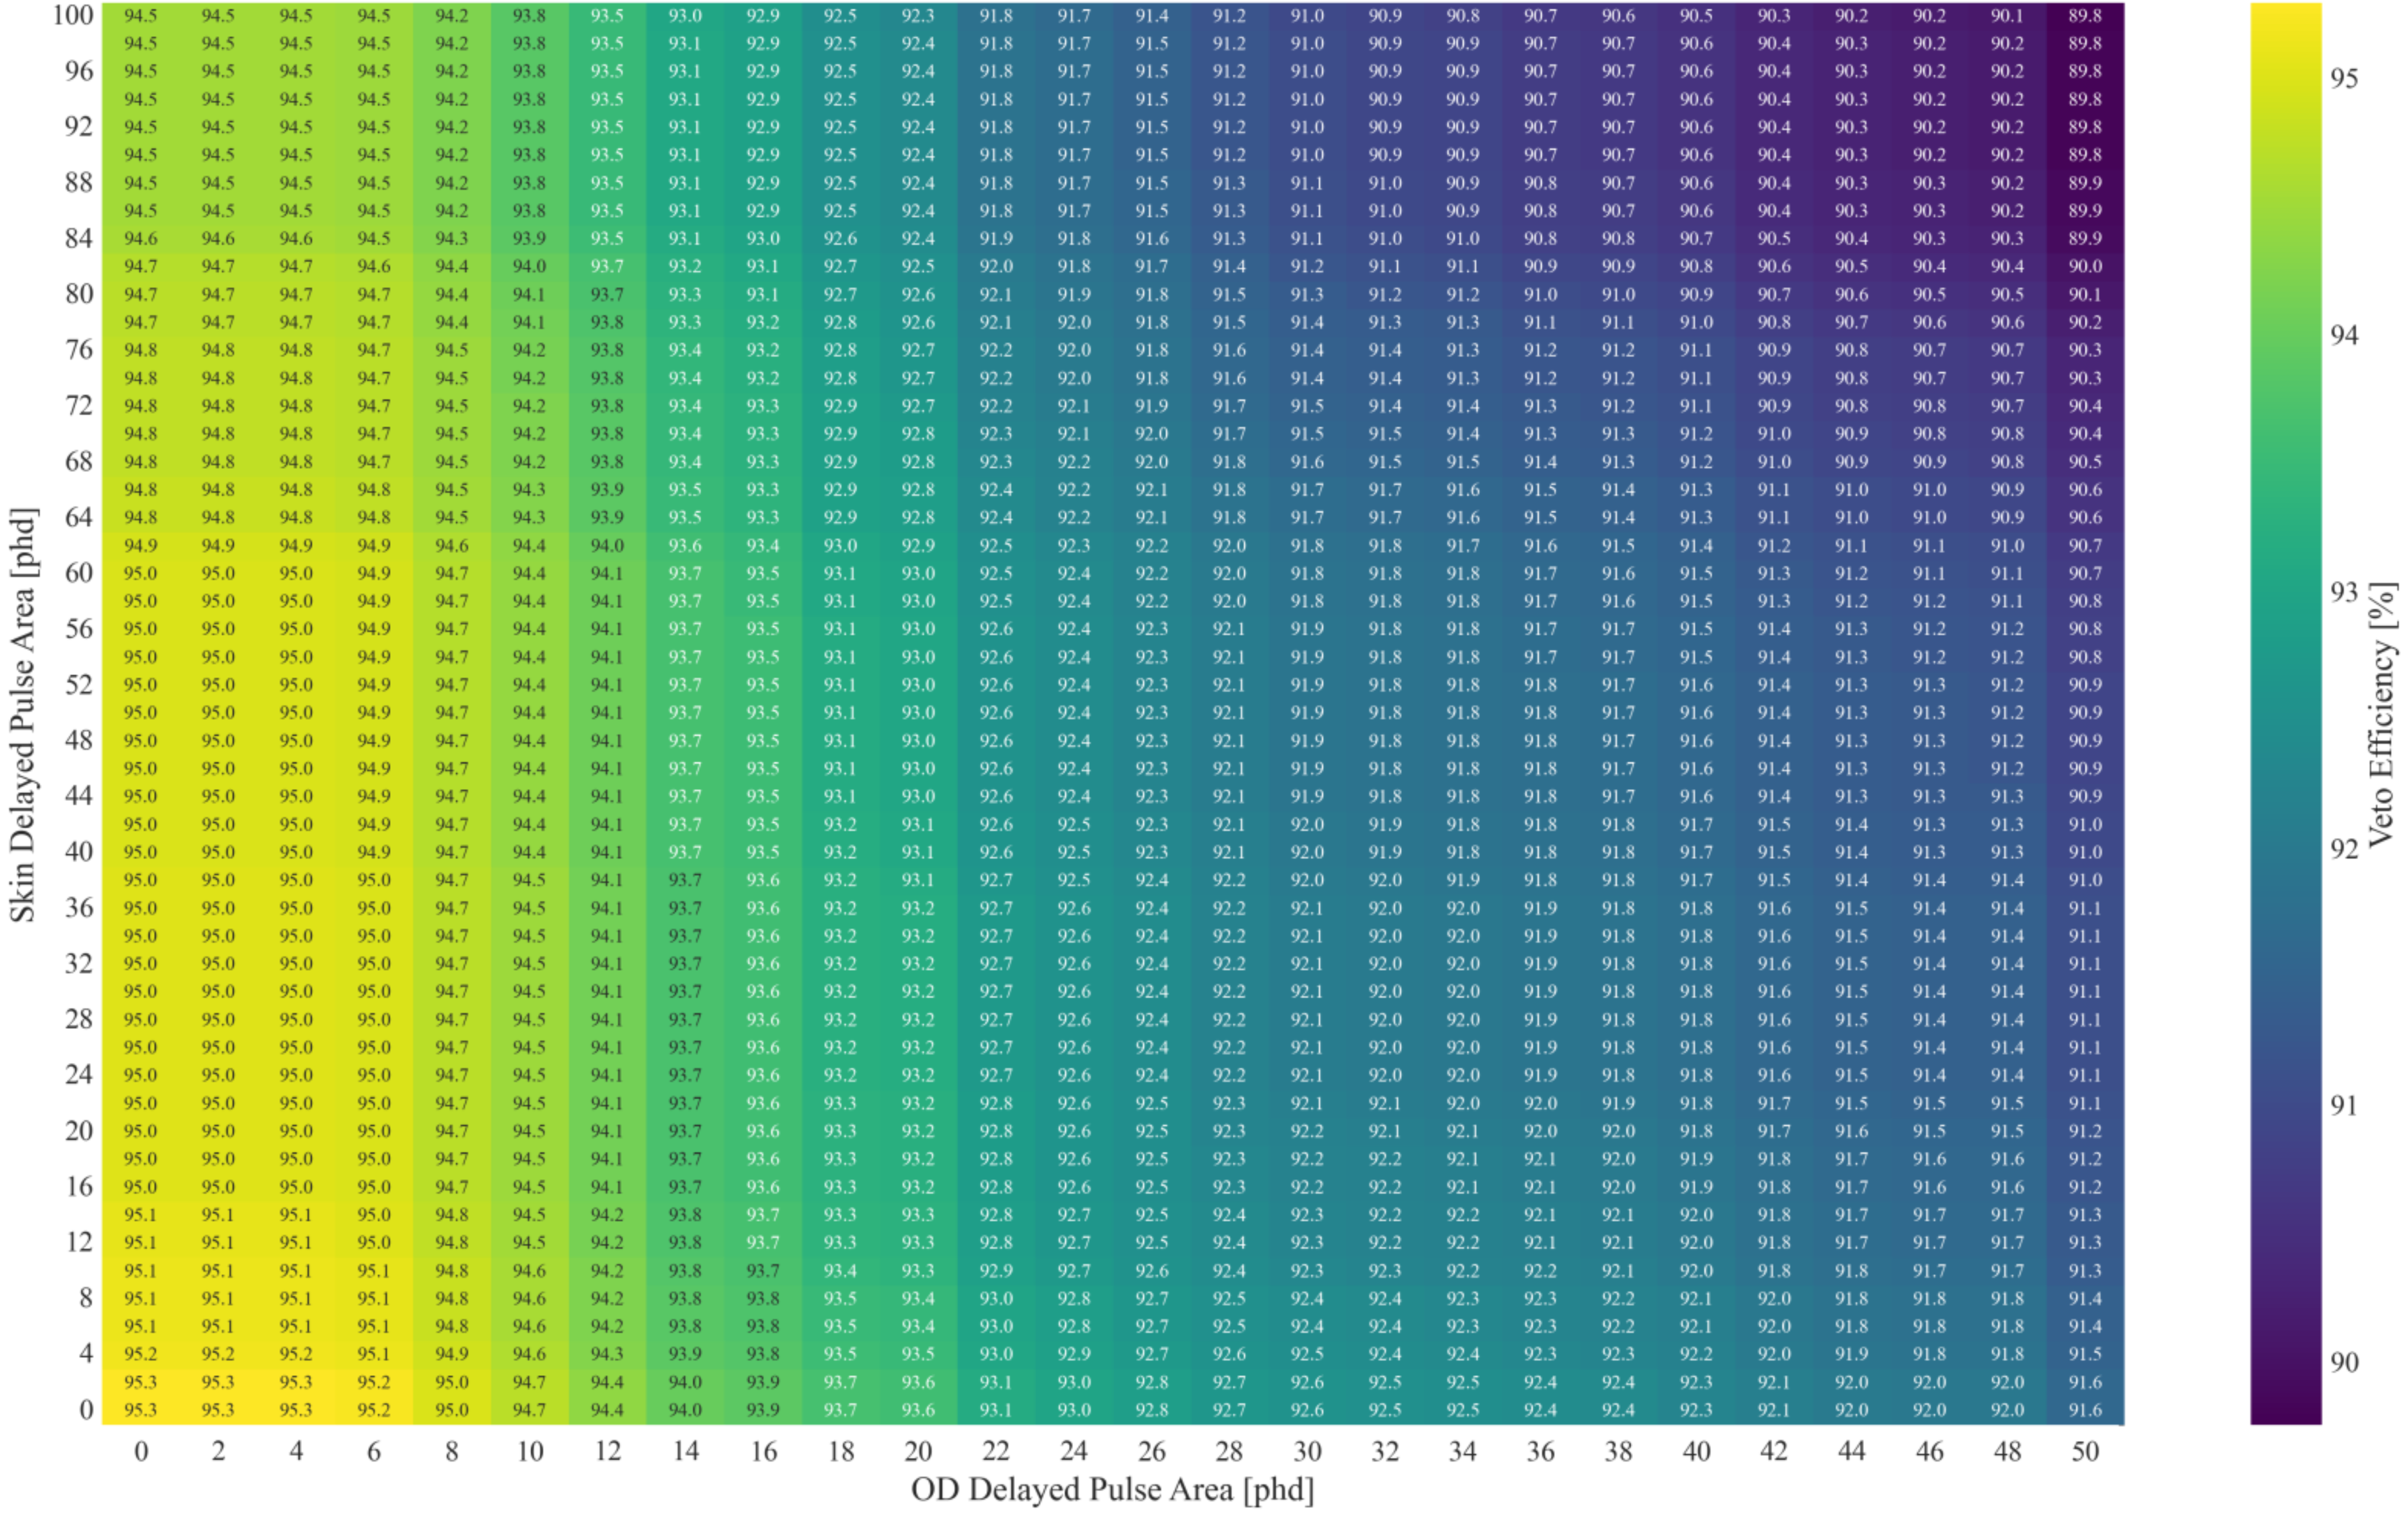
\includegraphics[width=\textwidth]{figures/VetoEfficiency/Heatmap600us_ODDelayedSkinDelayedThresholds.png}
	\caption{Heatmap used to determine optimal OD and Skin Delayed thresholds based on efficiency.
		The z-axis shows the efficiency associated with a given pulse area requirement for the delayed veto windows defined in \autoref{tab:VetoEff/sr3_veto_cuts}.
	}
	\label{fig:VetoEff/od_prompt_veto_heatmap}
\end{sidewaysfigure}

Compiling the heatmaps of efficiency and deadtime for established veto windows of the different criteria, thresholds were chosen to maximise efficiency whilst minimising dead time. An example plot used to determine this is shown in \autoref{fig:VetoEff/veto_cut_optimisation}.
For the WS2024 science run, the approach of trying to maintain the efficiency of WS2022 veto of $\sim$~89\%, whilst reducing the livetime impact was taken. It was determined that the efficiency could be matched to the veto efficiency achieved in the WS2022 science run whilst achieving a factor of two reduction in deadtime.

\noindent
The final cuts for the WS2024 science run are shown in \autoref{tab:VetoEff/sr3_veto_cuts}, with the WS2022 selection included for comparison.

\iffalse
\begin{sidewaysfigure}
	\centering
	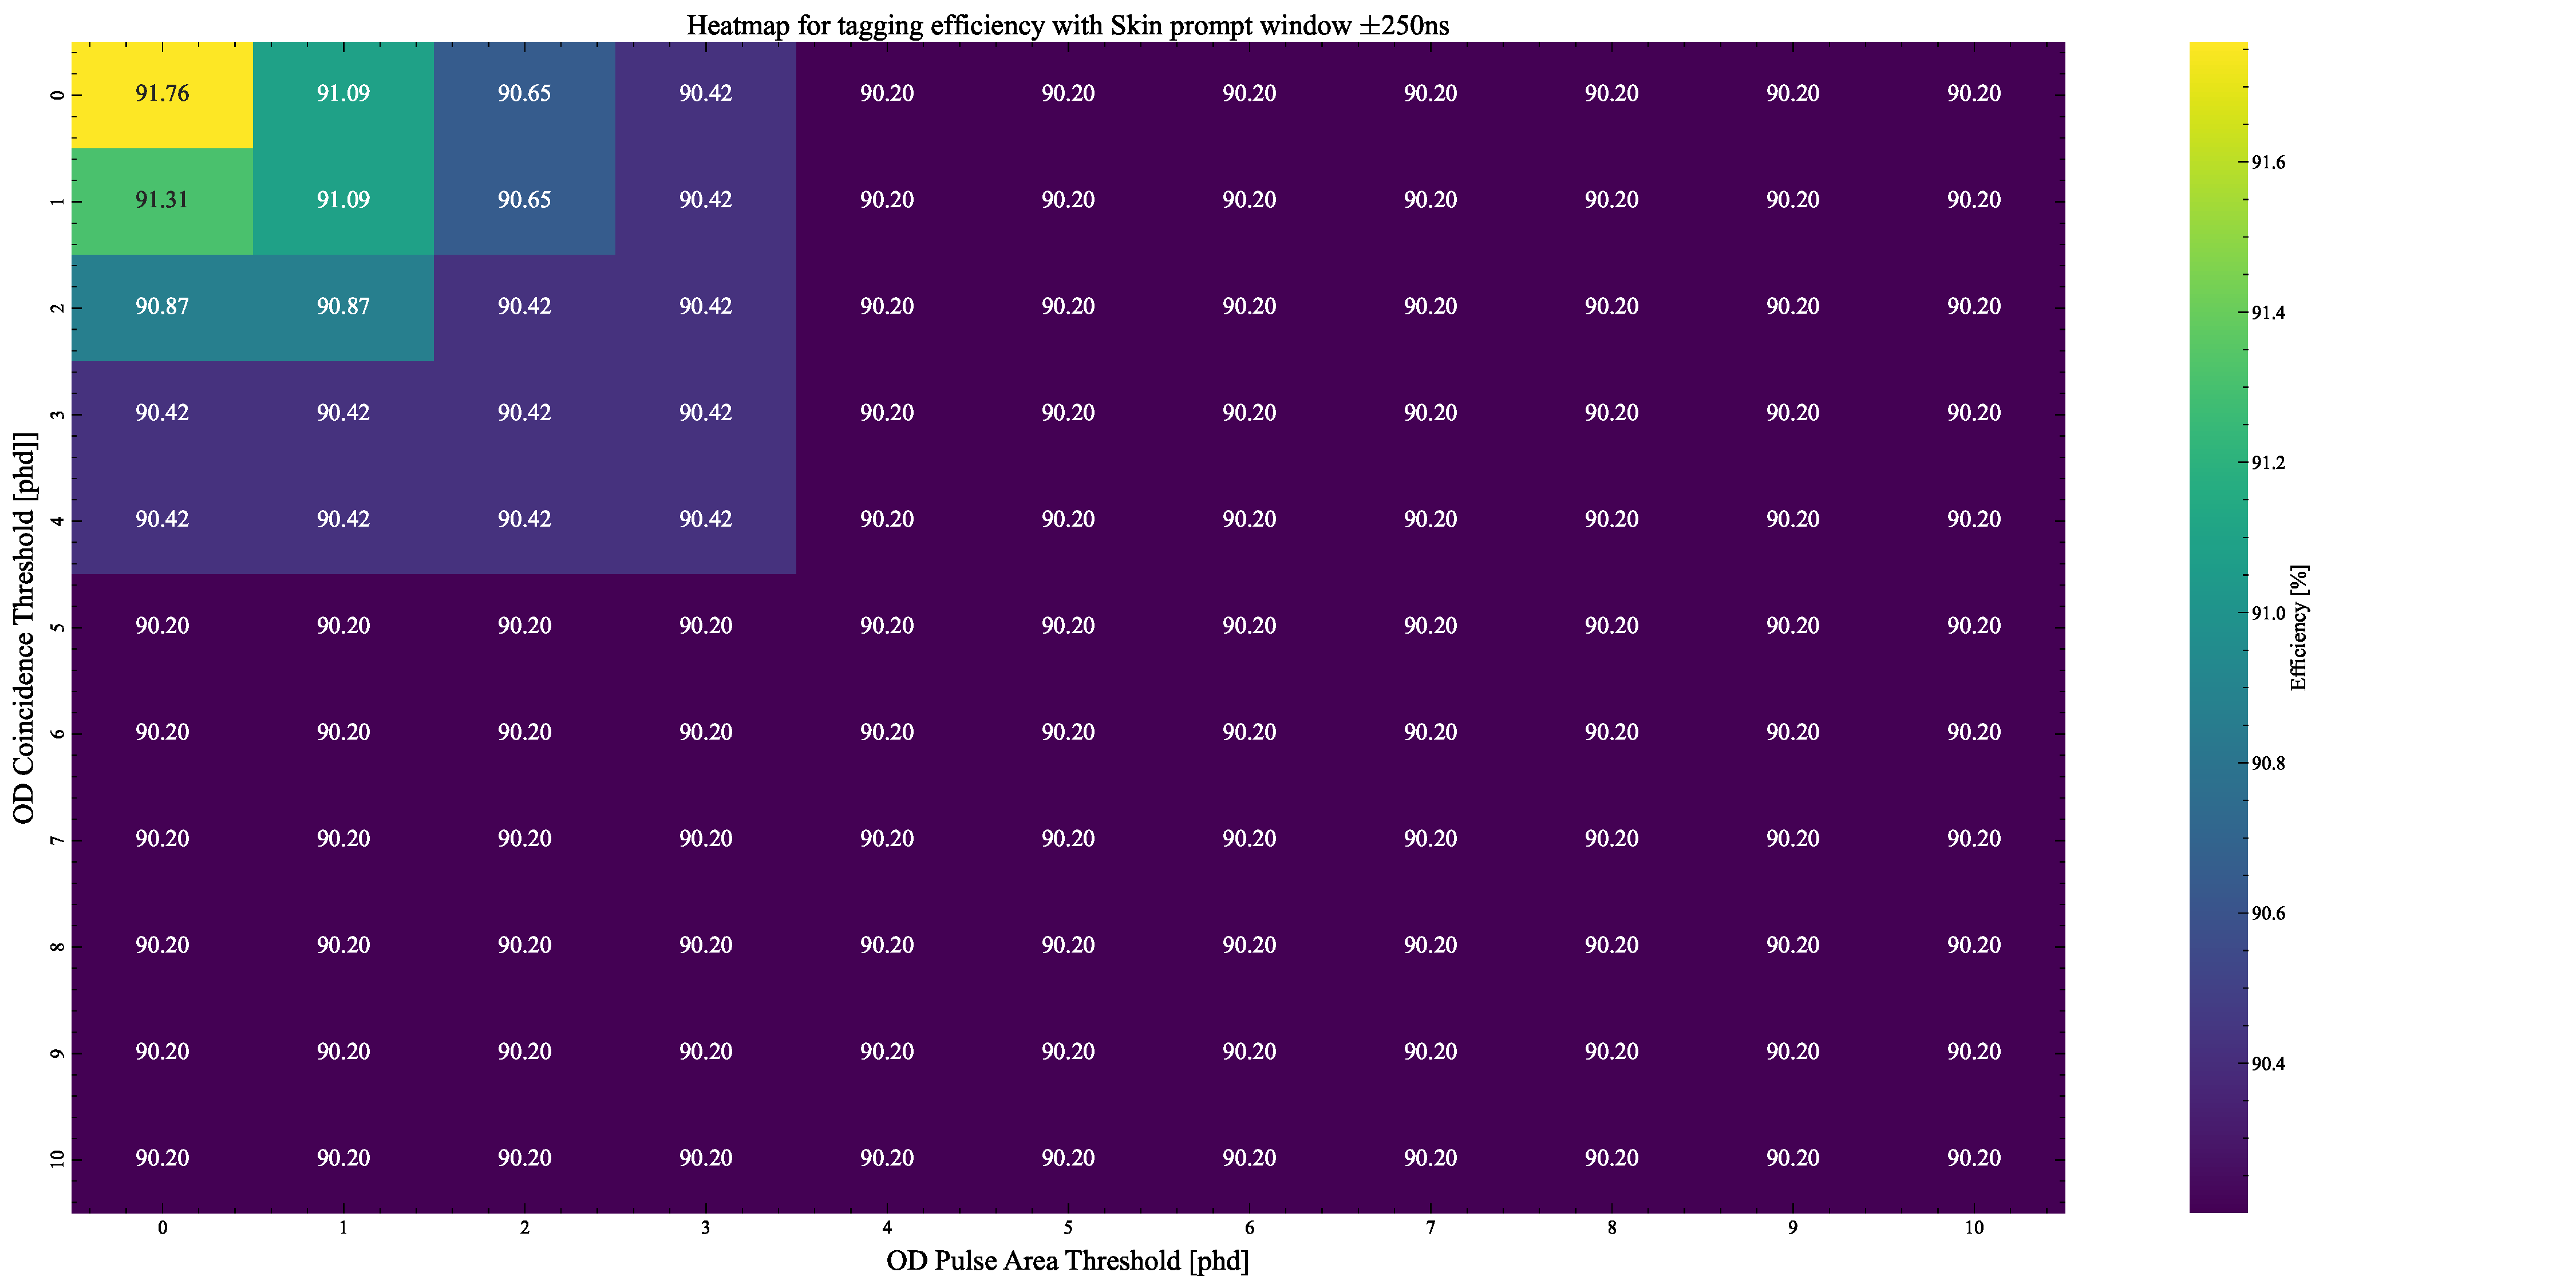
\includegraphics[width=\textwidth]{figures/VetoEfficiency/HeatmapSkinPACoinScanWindow500.pdf}
	\caption{Skin Prompt heatmap.
		In each bin, either the pulse coincidence or the pulse threshold has been varied.
		The z-axis shows the efficiency associated with a given pulse requirement.
		The veto time window considered is [-250, 250]ns.}
	\label{fig:VetoEff/skin_prompt_veto_heatmap}
\end{sidewaysfigure}
\begin{sidewaysfigure}
	\centering
	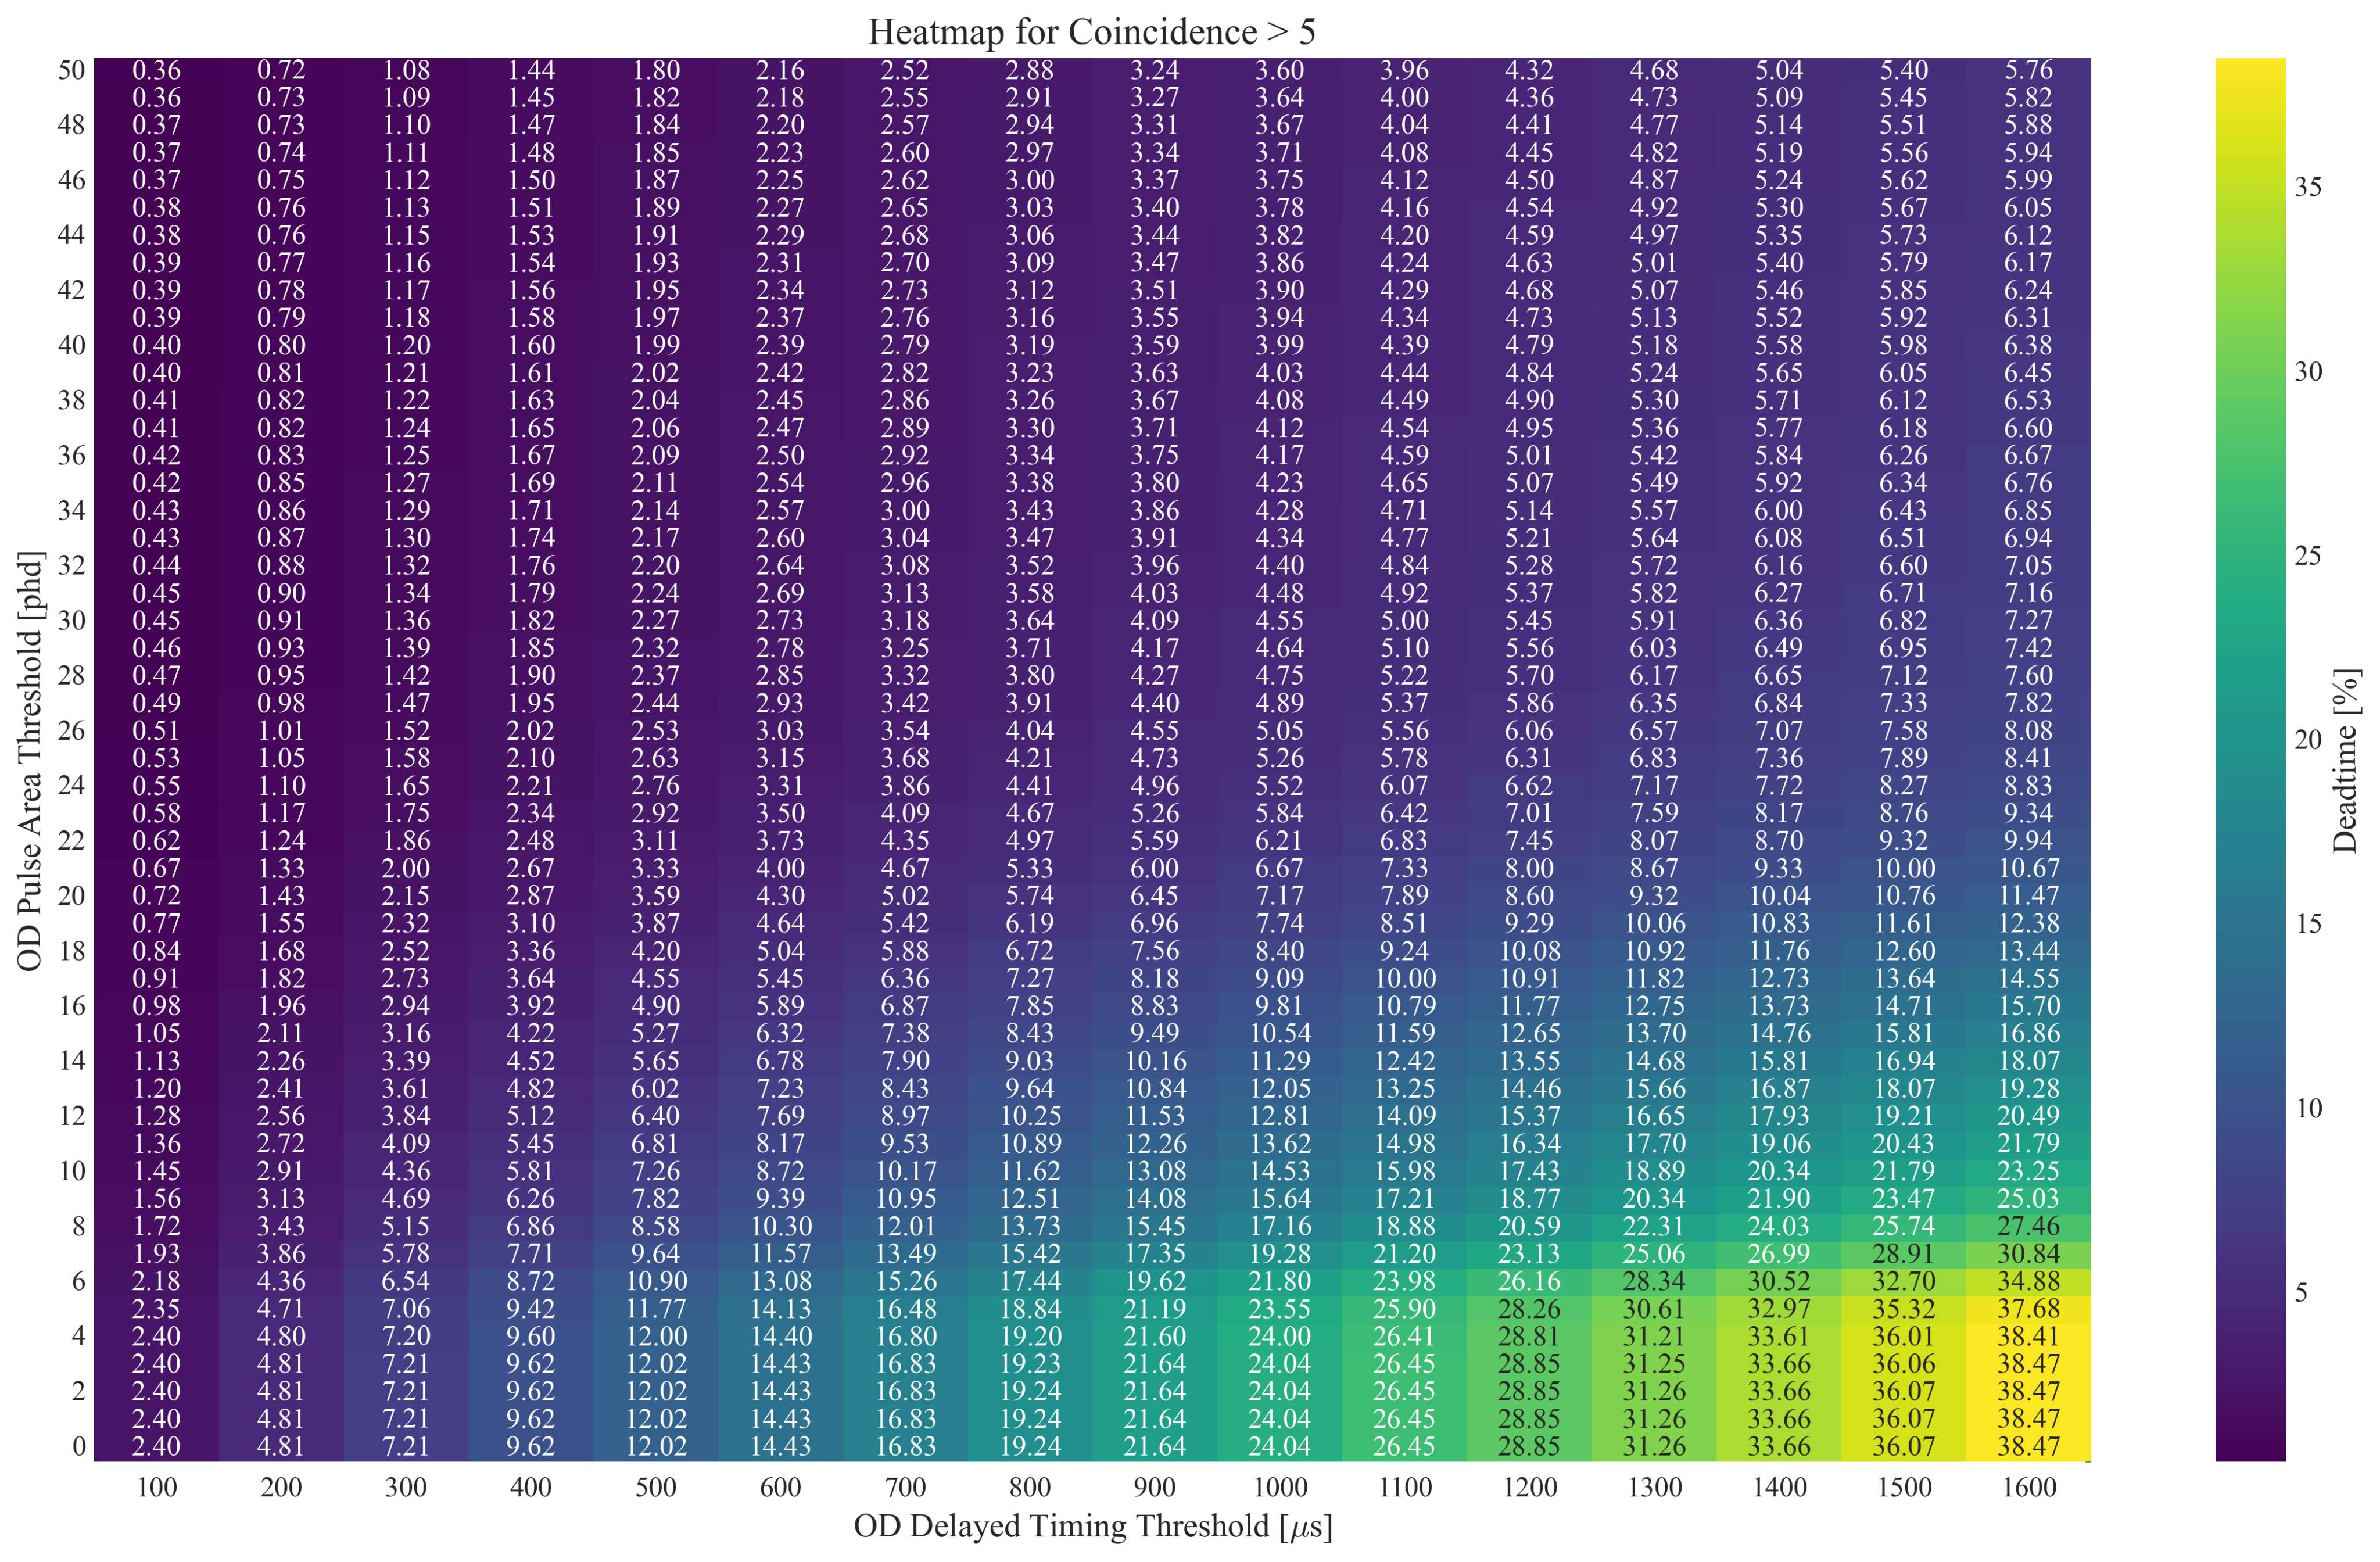
\includegraphics[width=\textwidth]{figures/VetoEfficiency/OD_Deadtime_thesis.png}
	\caption{OD Delayed heatmap.
		In each bin, either the veto window or the pulse threshold has been varied.
		The z-axis shows the deadtime associated with a given veto window and pulse threshold.
		In addition to the pulse area threshold, the pulse must have a coincidence greater than 5.}
	\label{fig:VetoEff/od_delayed_veto_heatmap}
\end{sidewaysfigure}
\begin{sidewaysfigure}
	\centering
	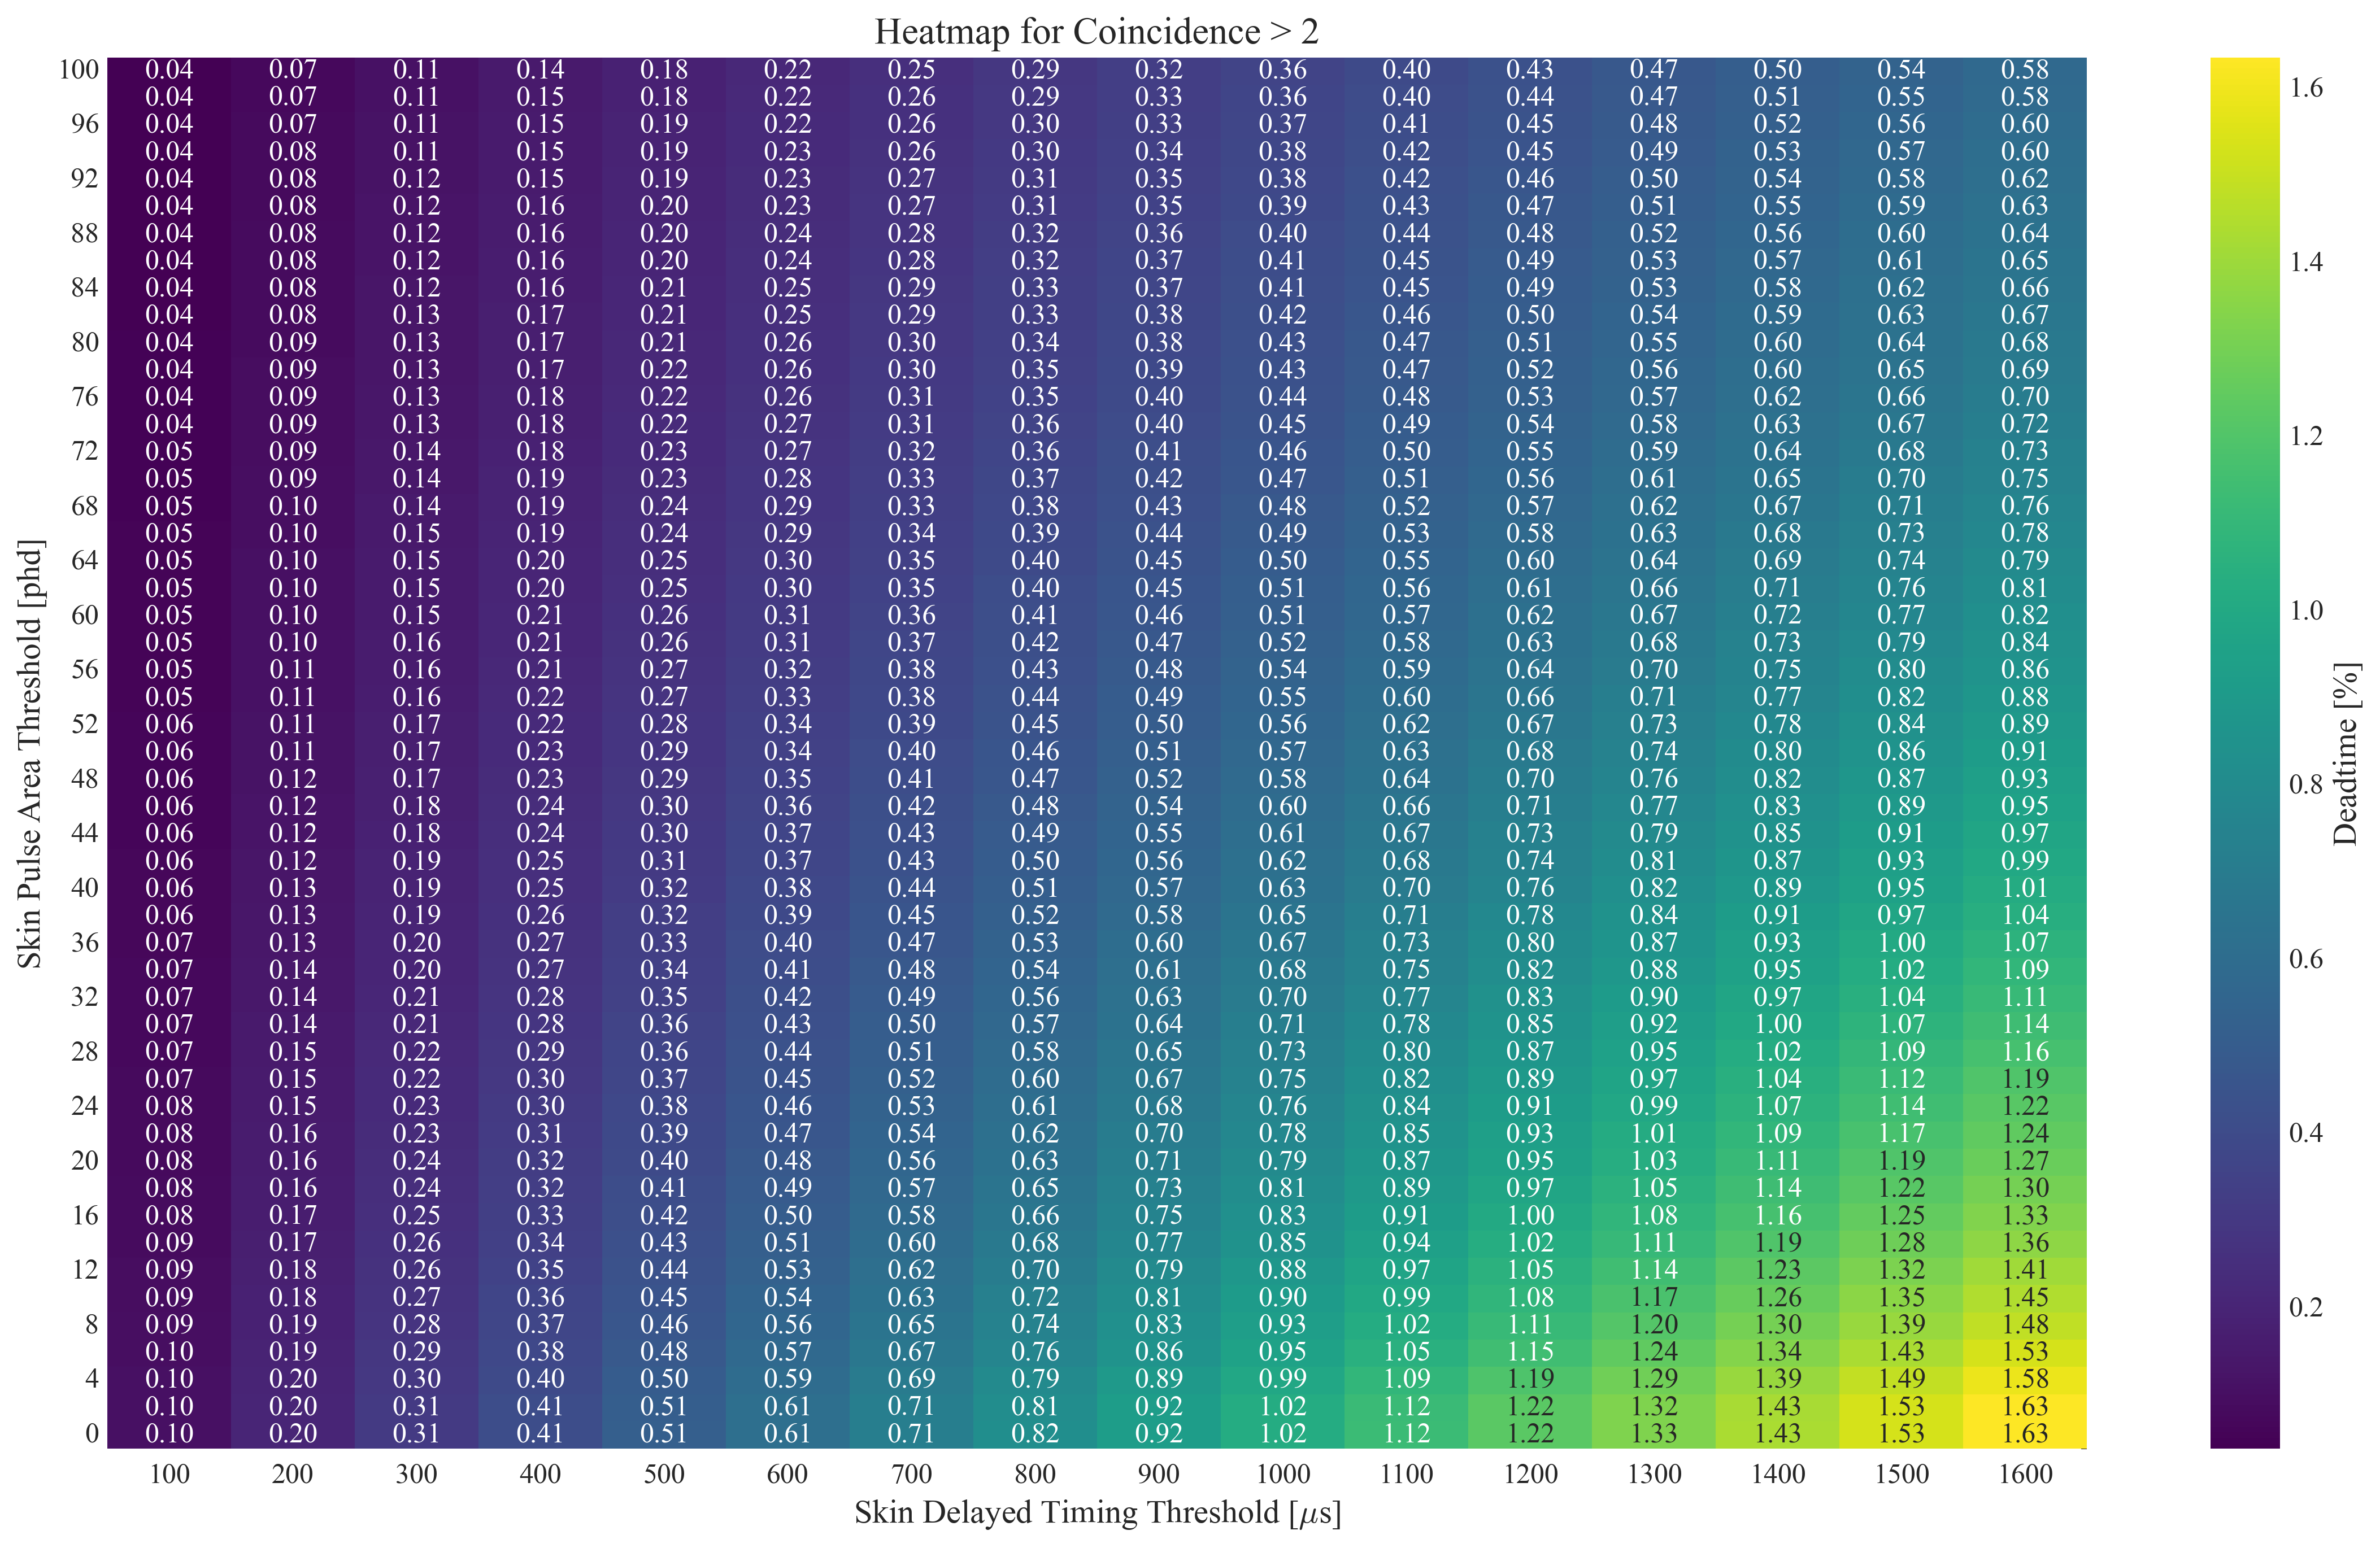
\includegraphics[width=\textwidth]{figures/VetoEfficiency/Skin_Deadtime_thesis.png}
	\caption{Delayed vetoes heatmap.
		In each bin, the OD pulse threshold or the Skin pulse threshold has been varied.
		The z-axis shows the veto efficiency associated with a given pulse thresholds.
		In addition to the pulse area threshold, the OD pulse must have a coincidence greater than 5, and the Skin pulse greater than 2.
		The veto window in this case is 500$\mu$s.}
	\label{fig:VetoEff/skin_delayed_veto_heatmap}
\end{sidewaysfigure}
\fi

\begin{figure}[!ht]
	\centering
	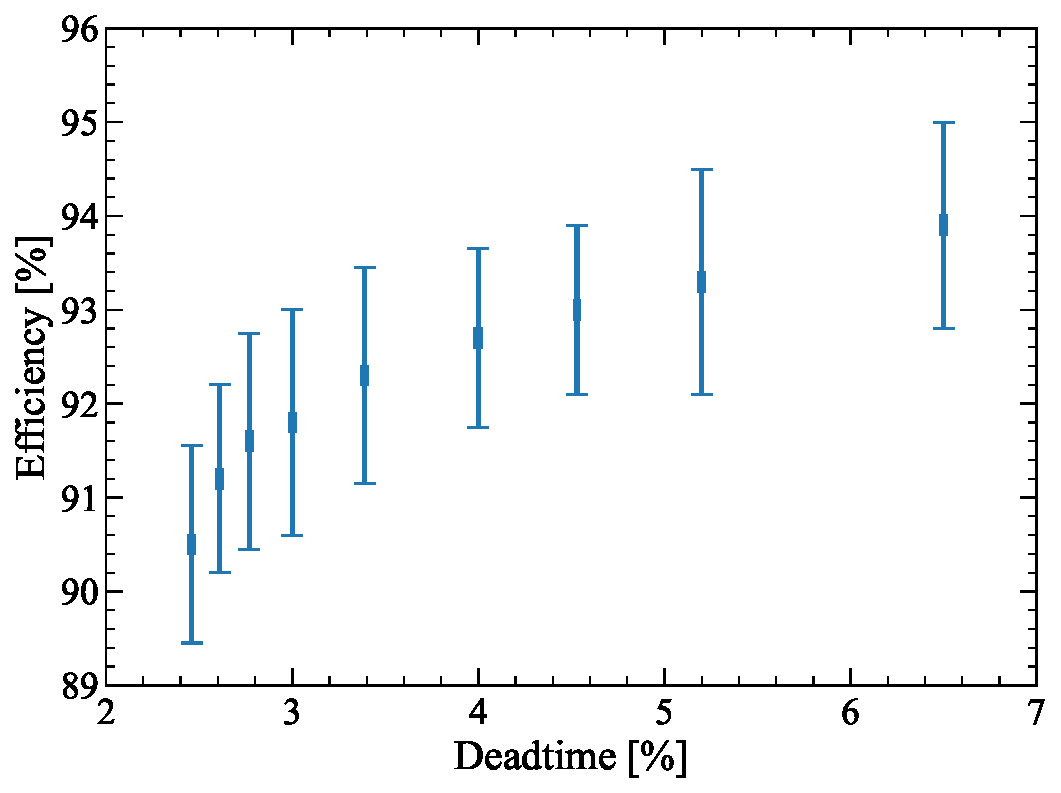
\includegraphics[width=0.6\textwidth]{figures/VetoEfficiency/DeadEffThresholdTest.pdf}
	\caption[Example plot used to highlight a number of considered cuts for the delayed Skin and OD pulse area thresholds for a 600~$\mu$s window.]{Example plot used to highlight a number of considered cuts for the delayed Skin and OD pulse area thresholds for a 600~$\mu$s window. The efficiency values have not been corrected for accidental coincidences. At each point, the numbers in brackets are the OD threshold pulse area, and the Skin threshold pulse area.}
	\label{fig:VetoEff/veto_cut_optimisation}
\end{figure}

\iffalse
\begin{figure}[!ht]
	\centering
	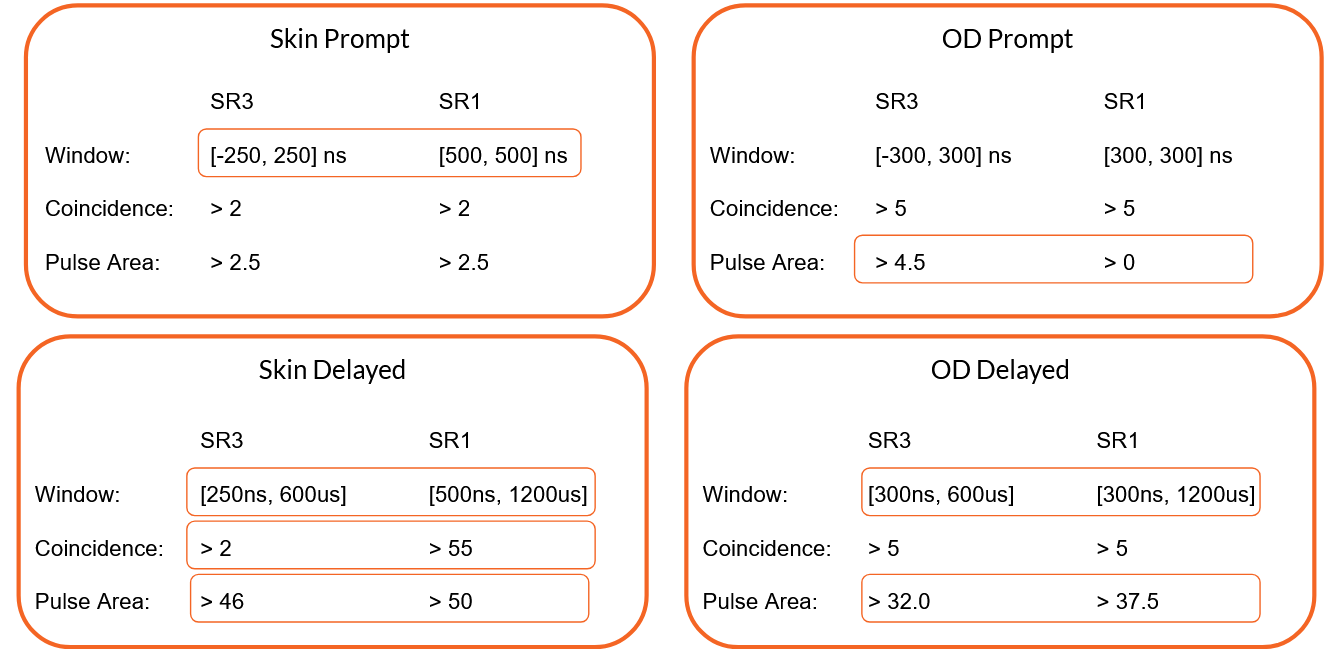
\includegraphics[width=0.9\textwidth]{figures/VetoEfficiency/sr3_cuts.png}
	\caption{Cuts determined to be optimal for the WS2024 science run.
		The WS2022 cuts are also included, where any modifications made to the selections is highlight accordingly.}
	\label{fig:VetoEff/sr3_veto_cuts}
\end{figure}
\fi

\begin{table}[!ht]
    \centering
    \caption{Cuts determined to be optimal for the WS2024 science run. The WS2022 cuts are also included, where any modifications made to the selections is shaded accordingly.}
    \label{tab:VetoEff/sr3_veto_cuts}
    \scalebox{0.9}{
    \begin{tabular}{|c|c|c||c|c|c|}
    \hline
    \multicolumn{3}{|c||}{\textbf{Skin Prompt}} & \multicolumn{3}{c|}{\textbf{OD Prompt}} \\
    \hline
    & WS2024 & WS2022 & & WS2024 & WS2022 \\
    \hline
    Window & \cellcolor[HTML]{cecece} [-250,250]~ns & \cellcolor[HTML]{cecece}[500,500]~ns & Window & [-300,300]~ns & [-300,300]~ns\\
    Coincidence&$>2$&$>2$&Coincidence&$>5$&$>5$\\
    Pulse Area & $>2.5$ & $>2.5$ & Pulse Area & \cellcolor[HTML]{cecece}$>4.5$ &\cellcolor[HTML]{cecece} $>0$ \\    
    \hhline{|===||===|}
    \multicolumn{3}{|c||}{\textbf{Skin Delayed}} & \multicolumn{3}{c|}{\textbf{OD Delayed}} \\
    \hline
    &WS2024&WS2022&&WS2024&WS2022\\
    \hline
    Window&\cellcolor[HTML]{cecece}[250~ns, 600~$\mu$s]&\cellcolor[HTML]{cecece}[500~ns, 1200~$\mu$s]&Window&\cellcolor[HTML]{cecece}[300~ns, 600~$\mu$s]&\cellcolor[HTML]{cecece}[300~ns, 1200~$\mu$s]\\
    Coincidence&\cellcolor[HTML]{cecece}$>2$&\cellcolor[HTML]{cecece}$>55$&Coincidence&$>5$&$>5$\\
    Pulse Area&\cellcolor[HTML]{cecece}$>46$&\cellcolor[HTML]{cecece}$>50$&Pulse Area&\cellcolor[HTML]{cecece}$>32.0$&\cellcolor[HTML]{cecece}$>37.5$\\
    \hline
    \end{tabular}}
\end{table}

\subsection{Deadtime stability}\label{sec:VetoEff/DeadtimeStability}
The stability of the induced deadtime for each of the veto selection windows over the WS2024 science run was assessed for stability by comparing the deadtime at monthly intervals. For each month, the rate of pulses in the Skin and OD, using the second half of the Random Trigger data was used; and the rate above the threshold, defined by the specific veto cut, was recorded. The stability of measured deadtime over the WS2024 science run is shown in \autoref{fig:VetoEff/deadtime_stability}.
The deadtime is then calculated as:
\begin{equation}
	\textrm{Dead Time [\%]} = 100 - (\lambda(x)\cdot t_{\text{vw}})
\end{equation}
where $\lambda(x)$ is the background rate above the veto threshold $x$, and $t_{\text{vw}}$ represents the veto window length measured in ns.
The conclusion that the deadtime is stable over the WS2024 science run was confirmed by looking at the rate of OD pulses above $200~\text{keV}$ (as defined by the WS2022 energy calibration) using the \lstinline{ODHealth} PREM module. No significant fluctuation was observed during WS2024 science run, shown in \autoref{fig:VetoEff/deadtime_stability_prem}.
\begin{figure}[!ht]
	\centering
	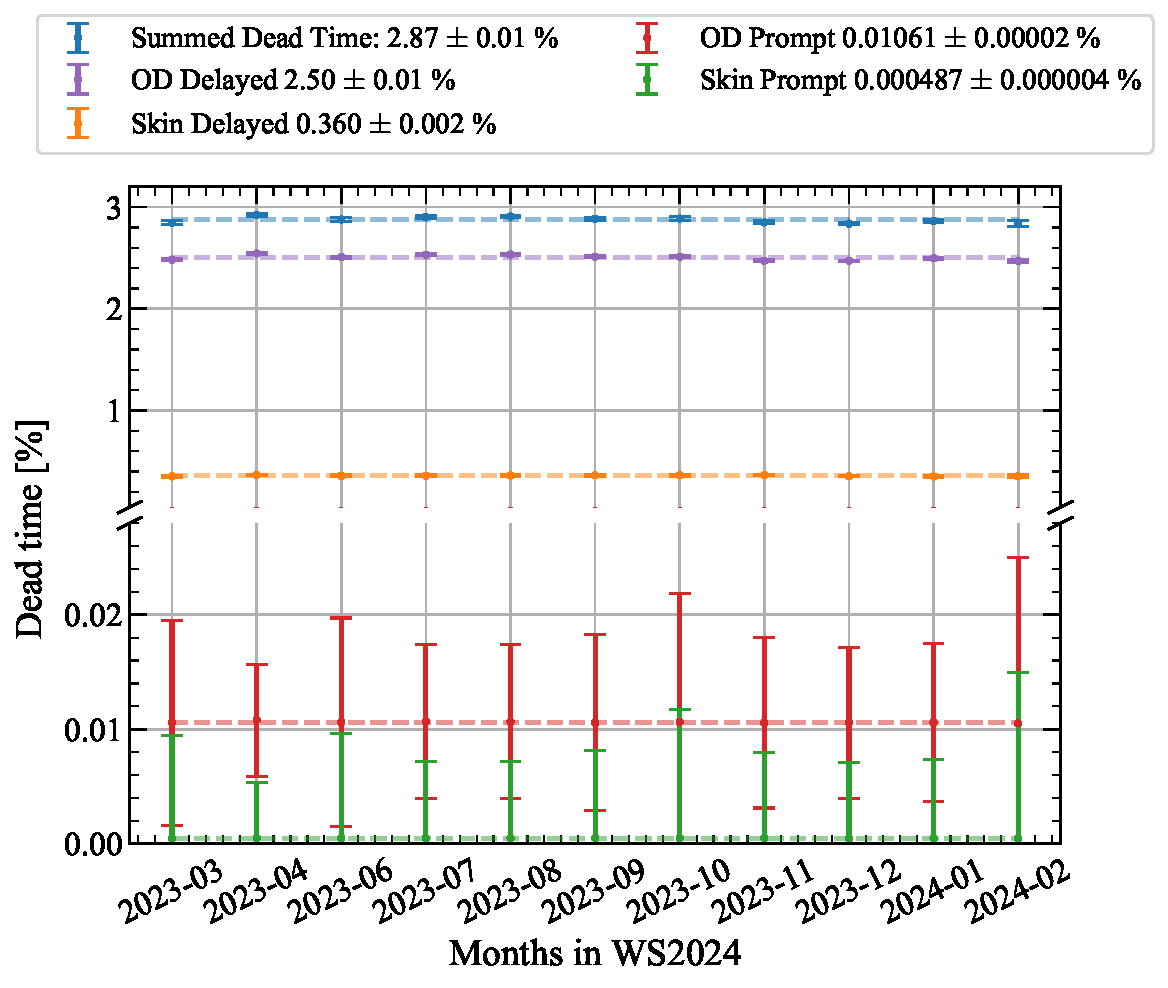
\includegraphics[width=0.7\textwidth]{figures/VetoEfficiency/SR3DeadTimeAll_withMean.pdf}
	\caption[Deadtime from the Skin and OD veto selection criteria during each month of WS2024 science run.]{Deadtime from the Skin and OD veto selection criteria during each month of WS2024 science run. The error shown in purely statistical and the mean across the science run is shown by a dashed line.}
	\label{fig:VetoEff/deadtime_stability}
\end{figure}
\begin{figure}[!ht]
	\centering
	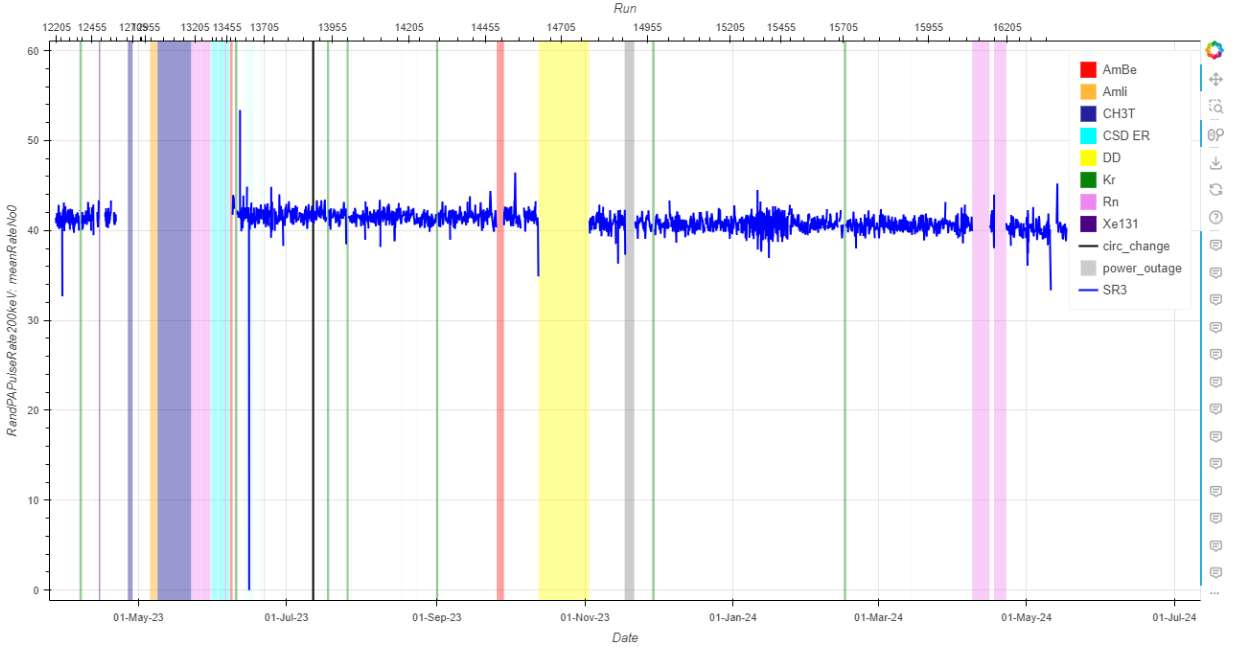
\includegraphics[width=\textwidth]{figures/VetoEfficiency/prem_od_stability.png}
	\caption[Rate of OD pulses above 200~keV over the WS2024 science run.]{Rate of OD pulses above 200~keV (as defined by WS2022 energy calibration) over the WS2024 science run. Various periods of calibration are indicated by the coloured regions. {\color{red}Ewan to help make new plot with sidebar.}}
	\label{fig:VetoEff/deadtime_stability_prem}
\end{figure}

\section{Neutron veto efficiency}\label{sec:VetoEff/efficiency}
In this section, the efficiency of tagging background neutrons using the Skin and OD detectors is calculated.
This is performed by calculating the efficiency on AmLi and DD calibration data and comparing to simulations.
The difference between efficiencies from simulations and data is then used to calculate an offset.
The efficiency is then calculated for detector NR simulations and the observed offset is used as a correction factor to estimate the tagging efficiency for events classified as detector NR \cite{LZ:2022ysc,LZ:2024zvo}.
The efficiency is defined as:
\begin{equation}\label{eqn:VetoEff/neutron_tagging_efficiency}
	\eta\;[\%] = \frac{\textrm{N. Events passing Analysis Cuts + Veto Cuts}}{\textrm{N. Events passing Analysis Cuts}} \times 100
\end{equation}
and the inefficiency is defined as $\cancel{\eta}=100-\eta$. For all veto efficiency calculations in this chapter, if a pulse in the Skin or OD passes any of the selections outlined in \autoref{tab:VetoEff/sr3_veto_cuts}, then the event is included in the number of events in the numerator of \autoref{eqn:VetoEff/neutron_tagging_efficiency}. The efficiency based on this decision logic is the \textit{total veto efficiency}.

Two additional efficiencies were investigated: \textit{delayed veto efficiency} defined as events where a pulse is observed that fulfils either of the Skin delayed or OD delayed selection criteria, denoted by $\eta_\text{delayed}$; and \textit{OD-delayed veto efficiency} defined as events where a pulse is observed that fulfils the OD delayed selection criteria, denoted by $\eta_\text{OD-delayed}$.

Unless otherwise stated, all veto efficiencies presented follow the \textit{total veto efficiency} logic.

\subsection{Neutrons from calibration sources}\label{sec:VetoEff/NeutronsFromCalibrationSources}
LZ utilises two neutron sources to measure the neutron tagging efficiencies of the veto detectors. AmLi sources are a compound of \textsuperscript{241}Am $\alpha$-radioactivity and \textsuperscript{7}Li produce low-energy neutron emission via nuclear $(\alpha,\text{n})$ reactions. Alphas from $^{241}$Am decay bombard the $^{7}$Li nuclei. This leads to a nuclear reaction of type \textsuperscript{7}Li$+\alpha \rightarrow$\textsuperscript{11}B\textsuperscript{*}. The excited \textsuperscript{11}B nucleus then decays to \textsuperscript{11}B via neutron emission. The neutrons produced by the AmLi sources have a maximum energy of $\sim1.5~\text{MeV}$ which results in a nuclear recoils depositing up to $\sim45~\text{keV}_{nr}$ of energy \cite{LZ:2024bsz}. Gamma radiation is also emitted in the \textsuperscript{241}Am decay to various states of \textsuperscript{237}Np and is an associated background to the reaction neutrons. The neutron to gamma ray emission ratio is 0.032 \cite{Sazzad:2023uqs}. The gamma ray background of the AmLi source is accounted for by the accidental correction factors described in \autoref{sec:VetoEff/AmLiAccCorrection}. The characterisation of the LZ AmLi sources is shown in Ref.~\cite{Sazzad:2023uqs}.

A deuterium-deuterium (DD) neutron generator is used to produce mono-energetic 2.46~MeV neutrons which result in nuclear recoils depositing up to $74~\text{keV}_{nr}$ of energy. Neutrons are produced by the DD generator as follows: Deuterium is ionized and turned into a plasma by a microwave. Deuterium ions in the plasma are accelerated towards a charged titanium-coated cooper target. D\textsuperscript{+} ions embed into the target form titanium deuteride. Subsequent D\textsuperscript{+} ions fuse to the embed ions and release neutrons via the D+D$\rightarrow$\textsuperscript{3}He+n. The generator is position outside of the water tank and neutrons are collimated and transmitted to the OCV through nitrogen purged conduits \cite{LZ:2024bsz}. The neutron production is pulsed to suppress the ER background rate and enables selection of events coincident with neutron production. Neutron pulsing decreases the impact of accidental coincidences which artificially increases the veto tagging efficiency. Accidental correction factors are still required as pulsing neutron production does not completely suppress accidental coincidences.

\subsubsection{AmLi}\label{sec:VetoEff/AmLi_Efficiency}
AmLi calibration data used is this study was taken during the May 2023 calibration campaign prior to the WS2024 science run. Events which were classified as single scatters by LZap and passed the selection outlined in \autoref{tab:VetoEff/amli_efficiency_cuts} were used for the study. Two additional cuts were applied to the calibration data:
\begin{enumerate}
	\item \textit{CSD tube position selection:} A circular cut on the reconstructed position of the SS S1 pulse in the TPC such that events from just one CSD tube are selected at a time. During the calibration campaign, sources were simultaneously deployed in each of the CSD tubes at equal heights (three separate height positions were used, $z=100~\text{mm},700~\text{mm},1300~\text{mm}$ relative to cathode at $z=0~\text{mm}$). Whereas separate simulations were produced with a single source in each CSD tube at three different heights (equal to the $z$-position used in the calibration campaign). 
    The circular cut selects events that have an SS S1 reconstructed position within a 50~mm radius of the CSD tube using the following equation:
    \begin{equation}\label{eqn:VetoEff/CSDSelection}
        \sqrt{(\text{S1}_x-\text{CSD}_x^i)^2+(\text{S1}_y-\text{CSD}_y^i)^2}<50
    \end{equation}
    where S1$_{x,y}$ is the reconstructed $(x,y)$-position of the S1 pulse in the SS and $\text{CSD}_{x,y}^i$ is the $(x,y)$-position of CSD where $i=1,2,3$ for each of the three CSD tubes.
    The boundaries of the cuts for each of the CSD tubes is shown in \autoref{fig:VetoEff/CSDSelection}. 
    \begin{figure}[!ht]
    \centering
        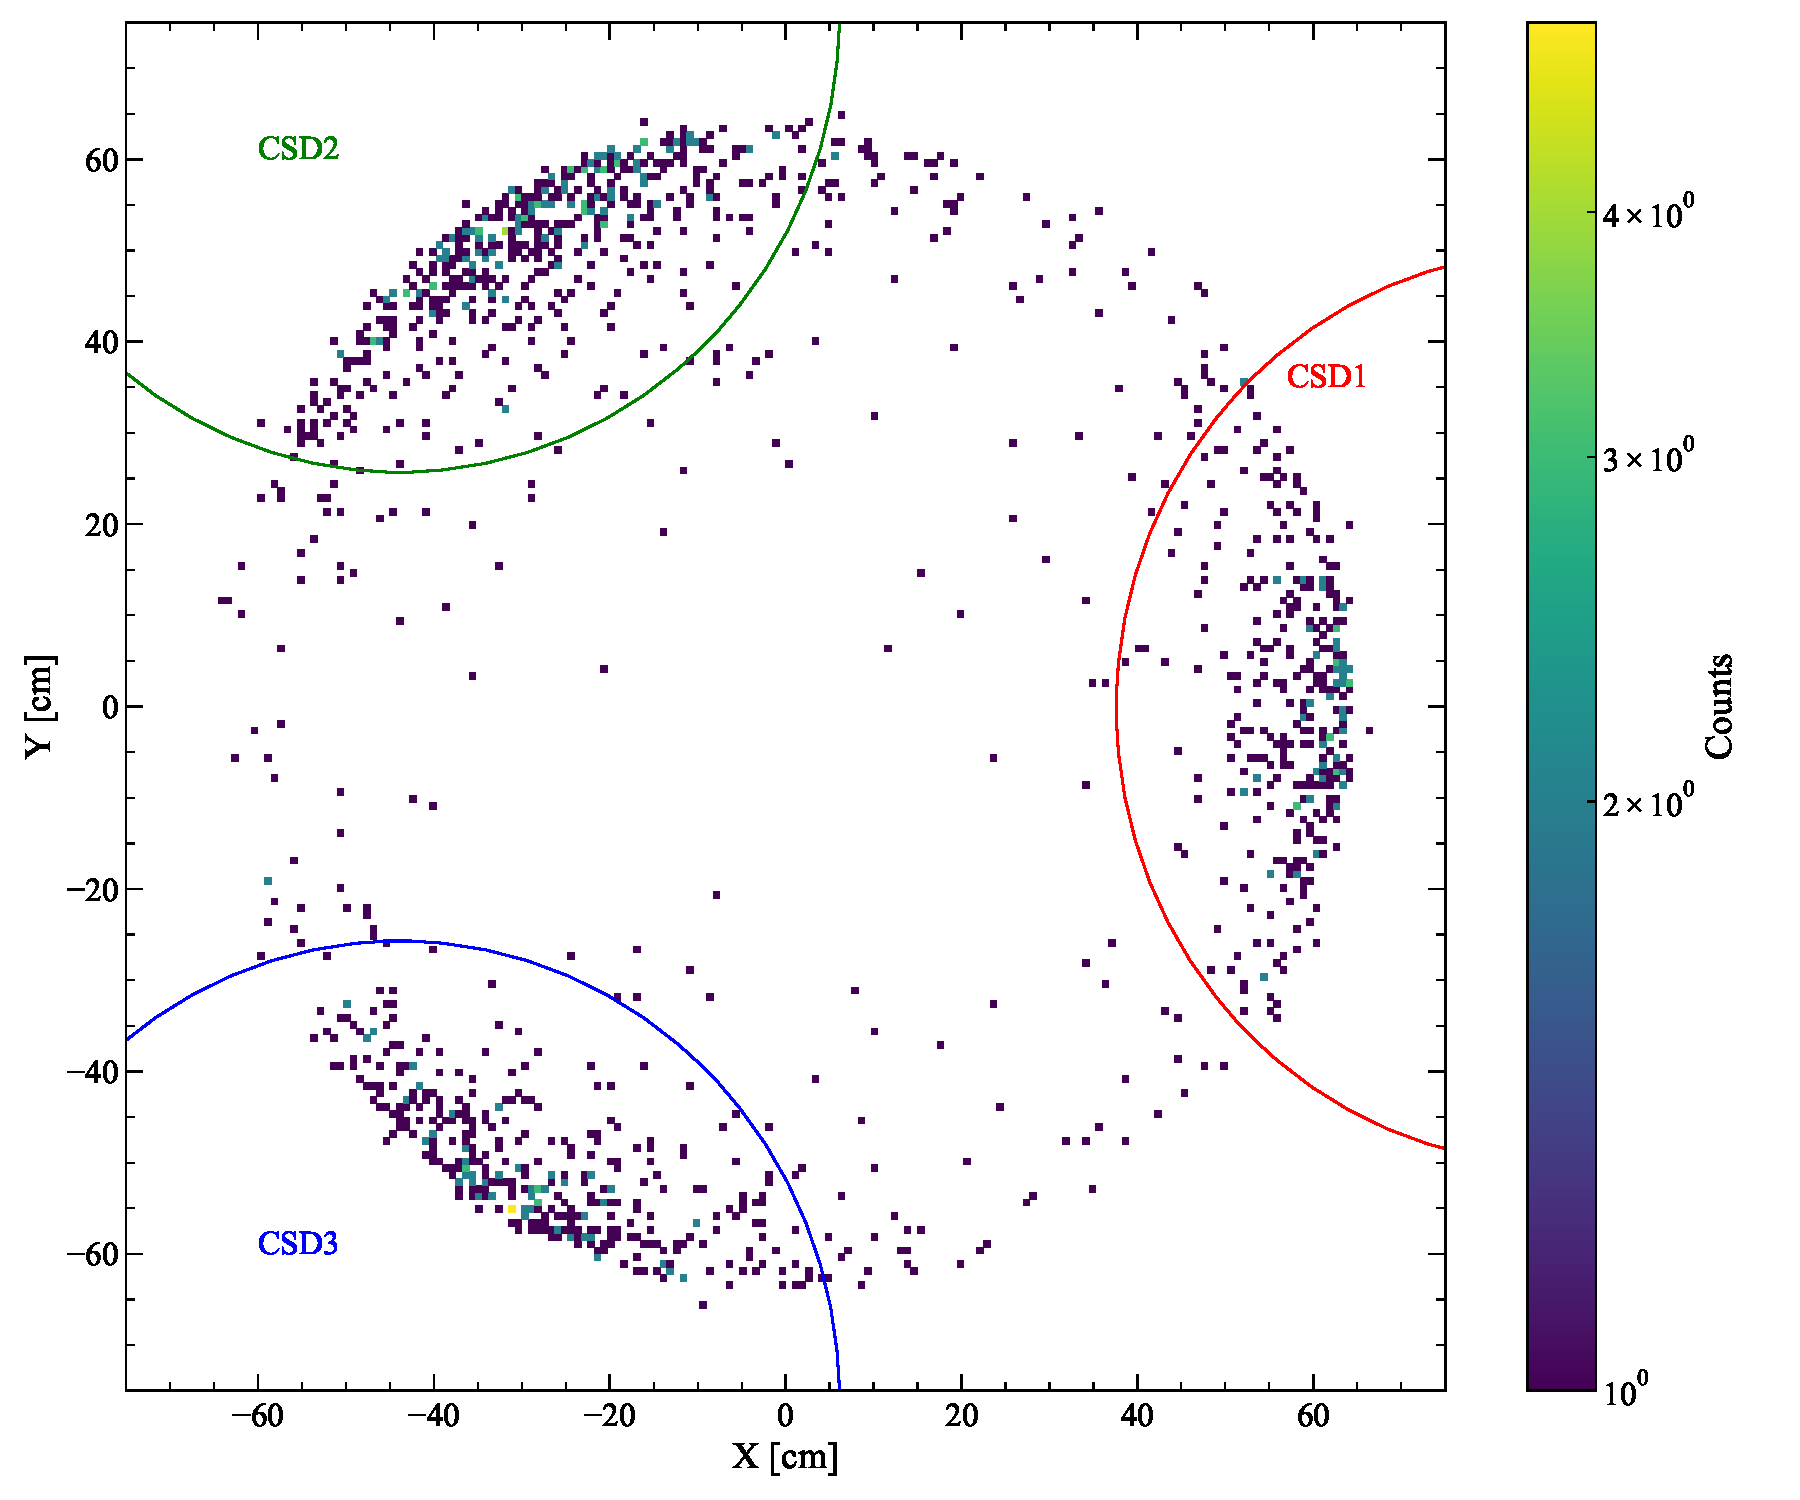
\includegraphics[width=0.7\textwidth]{figures/VetoEfficiency/CircularCSDCut.pdf}
        \caption{X-Y distribution of SS S1 pulses in the TPC for AmLi sources positioned at 700mm. Each of the circular cuts are overlaid on the plot.}
        \label{fig:VetoEff/CSDSelection}
    \end{figure}
    The position dependence of the veto efficiency can be examined by applying the CSD tube selection to data collected at different $z$-positions. The veto efficiency for different CSD tubes and $z$-positions is shown in \autoref{fig:VetoEff/VetoEffPositionDependence}.
    \begin{figure}[!ht]
    	\centering
    	\begin{subfigure}[b]{0.49\textwidth}
    		\centering
    		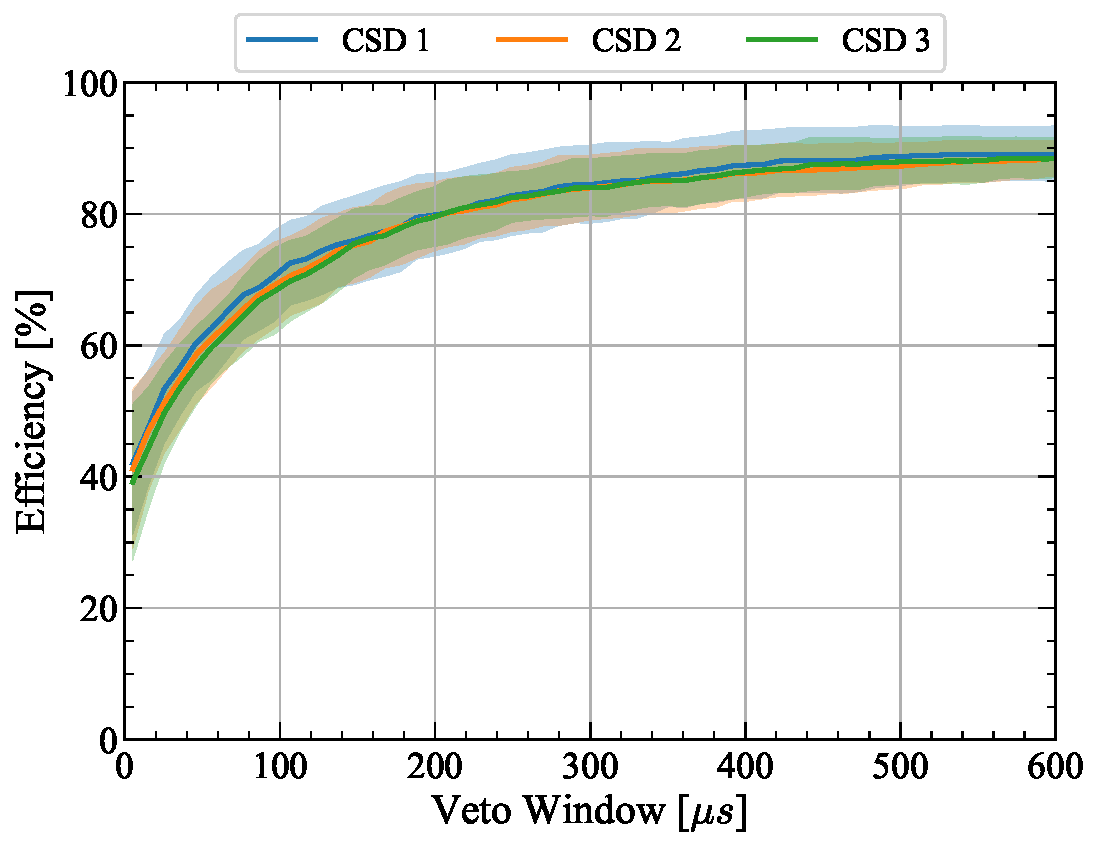
\includegraphics[width=\textwidth]{figures/VetoEfficiency/Eff_AmLi_Total_AllCSD.pdf}
    		\caption{}
            \label{fig:VetoEff/VetoEffPositionDependenceZPos}
    	\end{subfigure}
    	\hfill
    	\begin{subfigure}[b]{0.49\textwidth}
    		\centering
    		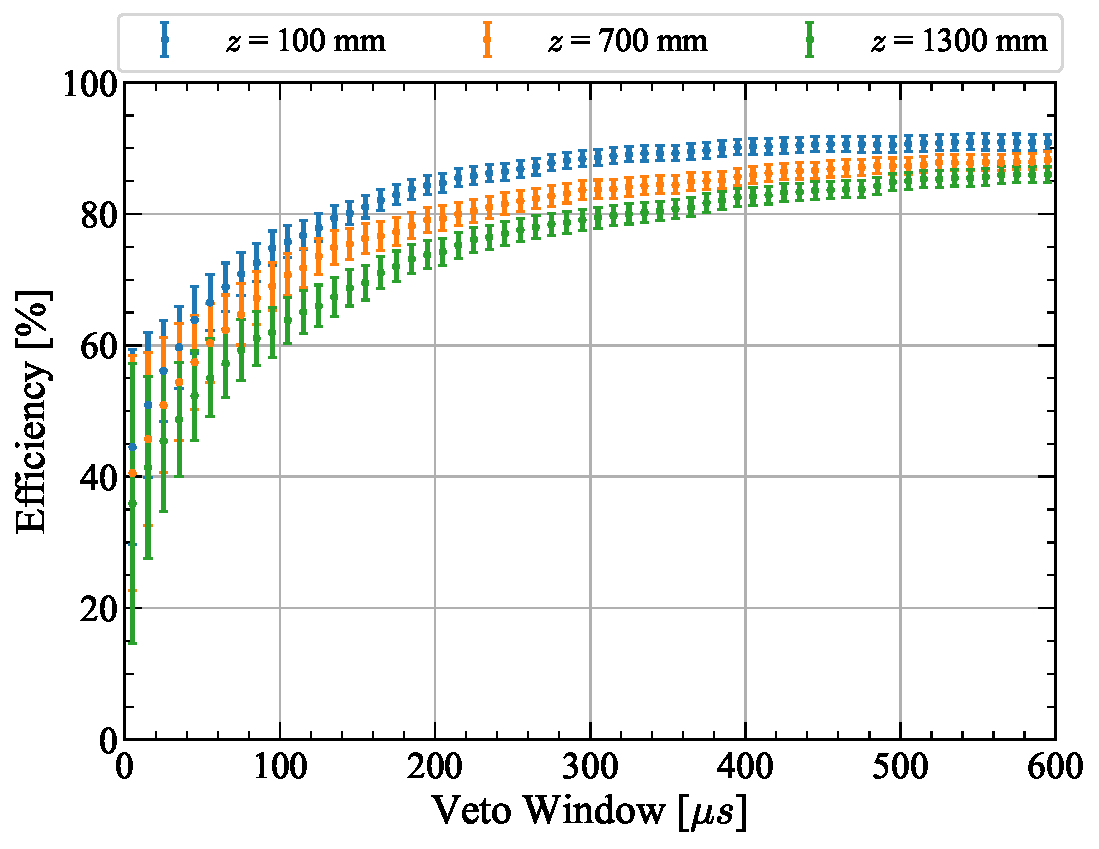
\includegraphics[width=\textwidth]{figures/VetoEfficiency/Eff_AmLi_Total_AllHeights.pdf}
            \caption{}
    		\label{fig:VetoEff/VetoEffPositionDependenceCSD}
    	\end{subfigure}
    	\caption{Position dependent veto efficiencies for different CSD tubes (left) and $z$-positions (right).}
    	\label{fig:VetoEff/VetoEffPositionDependence}
    \end{figure}
	A concern of this cut is that events towards the centre of the TPC are excluded. When the efficiency is averaged across different heights and CSD tube, the average can then be replicated in both data and simulation. 
    The position-averaged efficiency when the CSD cut is applied is $(88.21\pm1.03)\%$, whereas without the cut, the efficiency is $(88.25\pm1.22)\%$.
	The cut has $<5\%$ impact across the veto window and $<0.1\%$ impact at the 600~$\mu$s veto window threshold. This comparison is shown in \autoref{fig:VetoEff/CSDSelectionEffComp}.
    \begin{figure}[!ht]
    	\centering
    	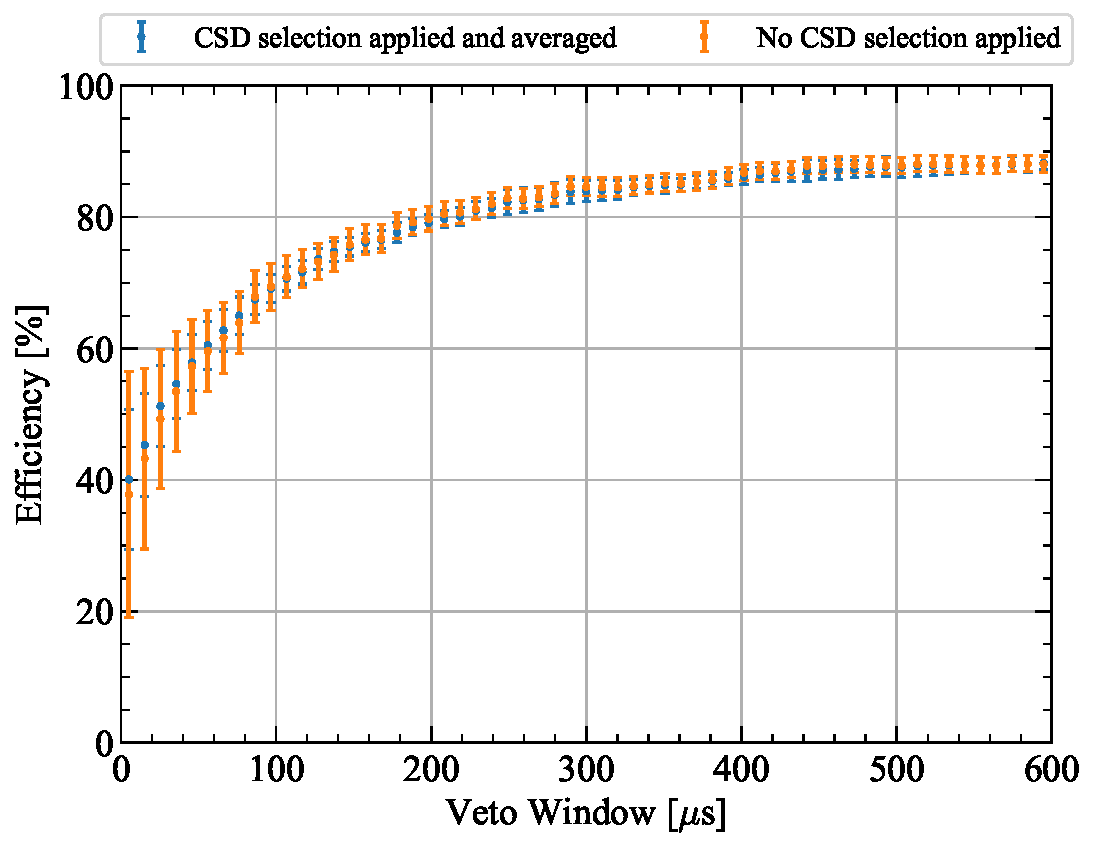
\includegraphics[width=0.7\linewidth]{figures/VetoEfficiency/CSDSelectionCheck.pdf}
    	\caption[CSD tube selection impact on veto efficiency.]{CSD tube selection impact on veto efficiency. The average veto efficiency for events which have a reconstructed position with 50~mm of a CSD tube (blue) is compared to veto efficiency of all events with no CSD selection applied. The cut has $<5\%$ impact across the veto window and $<0.1\%$ impact at the 600~$\mu$s veto window threshold.}
    	\label{fig:VetoEff/CSDSelectionEffComp}
    \end{figure}

	\item \textit{NR-band selection:} SS events which have a S1 and S2 pulse area which lie within 1-$\sigma$ of NR band mean are selected to be used in the veto efficiency calculation.
    The NR bands are generated using the Noble Element Simulation Technique (NEST) \cite{NEST2011} are shown in \autoref{fig:VetoEff/SR3NRBands}. 
    The selection is defined as:
    \begin{equation}\label{eqn:VetoEff/NRBandSelection}
        -1<\frac{log_{10}(\text{S2}_\text{obs.})-\overline{log_{10}(\text{S2})}(\text{S1}_\text{obs.})}{\sigma_{log_{10}(\overline{\text{S2}})}(\text{S1}_\text{obs.})}<1
    \end{equation}
    where $\text{S1}_\text{obs.}$ and $log_{10}(\text{S2}_\text{obs.})$ are the observed pulse areas from the SS, $\overline{log_{10}(\text{S2})}(\text{S1}_\text{obs.})$ is the mean S2 corresponding to a observed S1 with $\sigma_{log_{10}(\overline{\text{S2}})}(\text{S1}_\text{obs.})$ based on the NEST model. The purpose of this cut is to improve the purity of the selection. 
    \begin{figure}[!ht]
    \centering
    \begin{subfigure}[b]{0.49\textwidth}
        \centering
        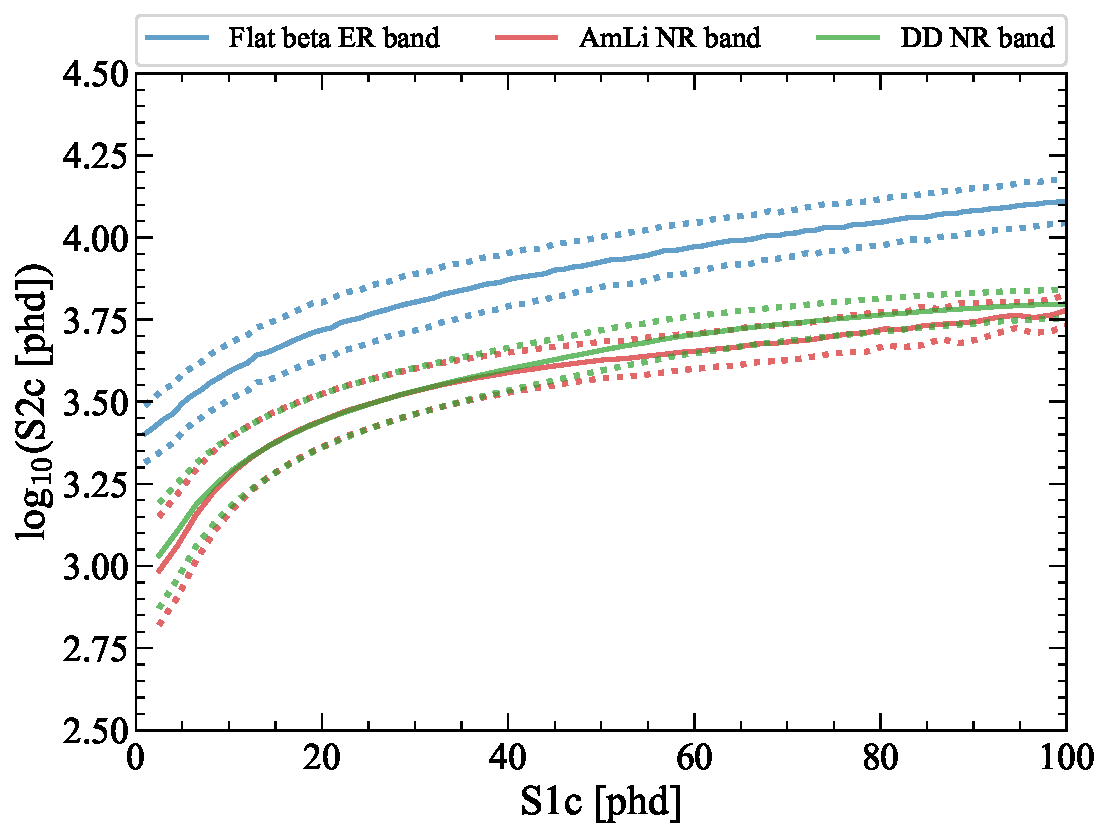
\includegraphics[width=\textwidth]{figures/VetoEfficiency/NRBands.pdf}
        \caption{}
        \label{fig:VetoEff/SR3NRBands}
    \end{subfigure}
    \hfill
    \begin{subfigure}[b]{0.49\textwidth}
        \centering
        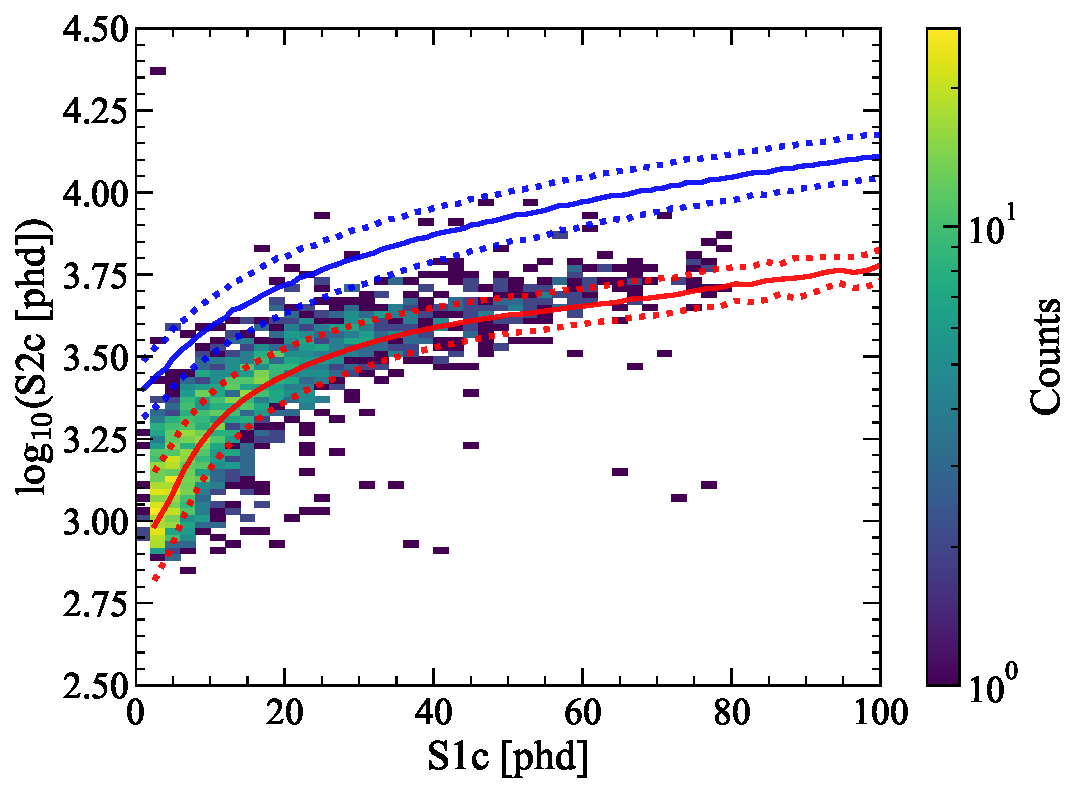
\includegraphics[width=\textwidth]{figures/VetoEfficiency/AmLi700_NRBands.pdf}
        \caption{}
        \label{fig:VetoEff/AmLi700_NRBands}
    \end{subfigure}
    \caption{\textbf{Left:} The NR band means (solid line) with 1-$\sigma$ boundaries (dashed lines) for AmLi and DD calibration sources and a flat beta ER band mean with 1-$\sigma$ boundary. Both NR and ER bands and 1-$\sigma$ boundaries were generated using NEST. \textbf{Right:} AmLi calibration data at $z=700~\text{mm}$ with the corresponding NR band mean and 1-$\sigma$ boundary overlaid.}
    \label{fig:VetoEff/SR3NRBands&AmLi700mmData}
\end{figure}
\end{enumerate}

\subsubsection{Accidental correction factor calculation}\label{sec:VetoEff/AmLiAccCorrection}
When determining the veto tagging efficiency a correction factor must be applied to the measured efficiency ($\eta_\text{obs.}$) to account for the accidental coincidences from neutrons and gamma rays\footnote{Neutrons which are associated with accidental coincidences are produced via additional $(\alpha,\text{n})$ reactions of the AmLi source whilst gamma rays are produced from neutron capture on Gd and H in the GdLS. A small percentage of gamma rays a produced by the $\alpha$ decay of \textsuperscript{241}Am \cite{Sazzad:2023uqs}.} with single scatter in the TPC which can artificially enhance the apparent measured tagging efficiency.
To calculate the accidental correction factors the veto inefficiency is defined as $\cancel{\eta}=M/N$, where $N$ represents the number of events which contain a single scatter nuclear recoil observed in the TPC and $M$ corresponds to the number of events where a single scatter nuclear recoil is observed in the TPC but no pulse is observed in the Skin or the OD that satisfies the veto requirements, this event is not vetoed.
The veto efficiency is subsequently defined as $\eta=1-\cancel{\eta}$.
The effect of the accidental coincidences has on the veto inefficiency is defined by the following process.
If a neutron scatters in the TPC, and is not detected by the veto detectors, instead there is an accidental coincidence of a gamma or neutron from the AmLi sources alongside TPC event. This is not included in the number of events, $M$.
The probability this occurrence is defined as $1-P_a(0)$, where $P_a(0)$ is the probability of observing zero accidental pulses in one of Skin or OD coincidence windows.
Using this probability and the number of events $M$ and $N$, the true inefficiency ($\cancel{\eta}_\text{true}$) is defined through the following derivation:
\label{eqn:Accidentals}
    \begin{align}
	M_\text{obs.}&=M_\text{true}-M_\text{true}\cdot(1-P_a(0))\\
	\Rightarrow M_\text{obs.}&=M_\text{true}\cdot P_a(0)\\
    \therefore M_\text{true}&=\frac{M_\text{obs.}}{P_a(0)}\\
	\cancel{\eta}_\text{true}=\frac{M_\text{true}}{N}&\text{ and }\cancel{\eta}_\text{obs.}=\frac{M_\text{obs.}}{N}\\
    \therefore \cancel{\eta}_\text{true}&=\frac{\cancel{\eta}_\text{obs.}}{P_a(0)}
    \end{align}
where $M_\text{obs.}$ is the number of events where no pulses have been observed in any of the veto windows and $M_\text{true}$ is the number of events where at least one pulse has been observed in one of the veto windows due to an accidental coincidence.
This leads to a final inefficiency:
\begin{equation}
	\cancel{\eta}_\text{true} = \frac{\cancel{\eta}_\text{obs.}}{1-P_a(>0)_{\text{any window}}}=\frac{\cancel{\eta}_\text{obs.}}{P_a(0)_{\text{all windows}}}
\end{equation}
$1-P_a(>0)_{\text{any window}}$ is determined directly using the post-trigger window of randomly triggered events and any pulse in any of the veto windows is counted. $P_a(0)_{\text{all windows}}$ for all detector windows is logically equivalent to $P_a(0)$ for a one detector, one window case.

The accidental correction is correlated with the length of the veto window. Scans over the entire delayed veto window in 10~$\mu$s steps to observe the change in the correction factor over time is shown in \autoref{fig:VetoEff/SR3AmLi_700mm_Corrections}. The probability of observing zero accidental pulses in the veto detector decreases with increasing veto window size. The probability of observing a coincident neutron from the AmLi or gamma from neutron capture on Gd and H in the GdLS increases with veto window size. At $600~\mu\text{s}$, $P_a(0)_{\text{all windows}}=0.79\pm0.03$. 
The impact of the accidental correction when applied to the observed efficiency is shown in \autoref{fig:VetoEff/AmLiAccidentalCorrectionImpact}.

\begin{figure}[!ht]
    \centering
    \begin{subfigure}[b]{0.49\textwidth}
        \centering
        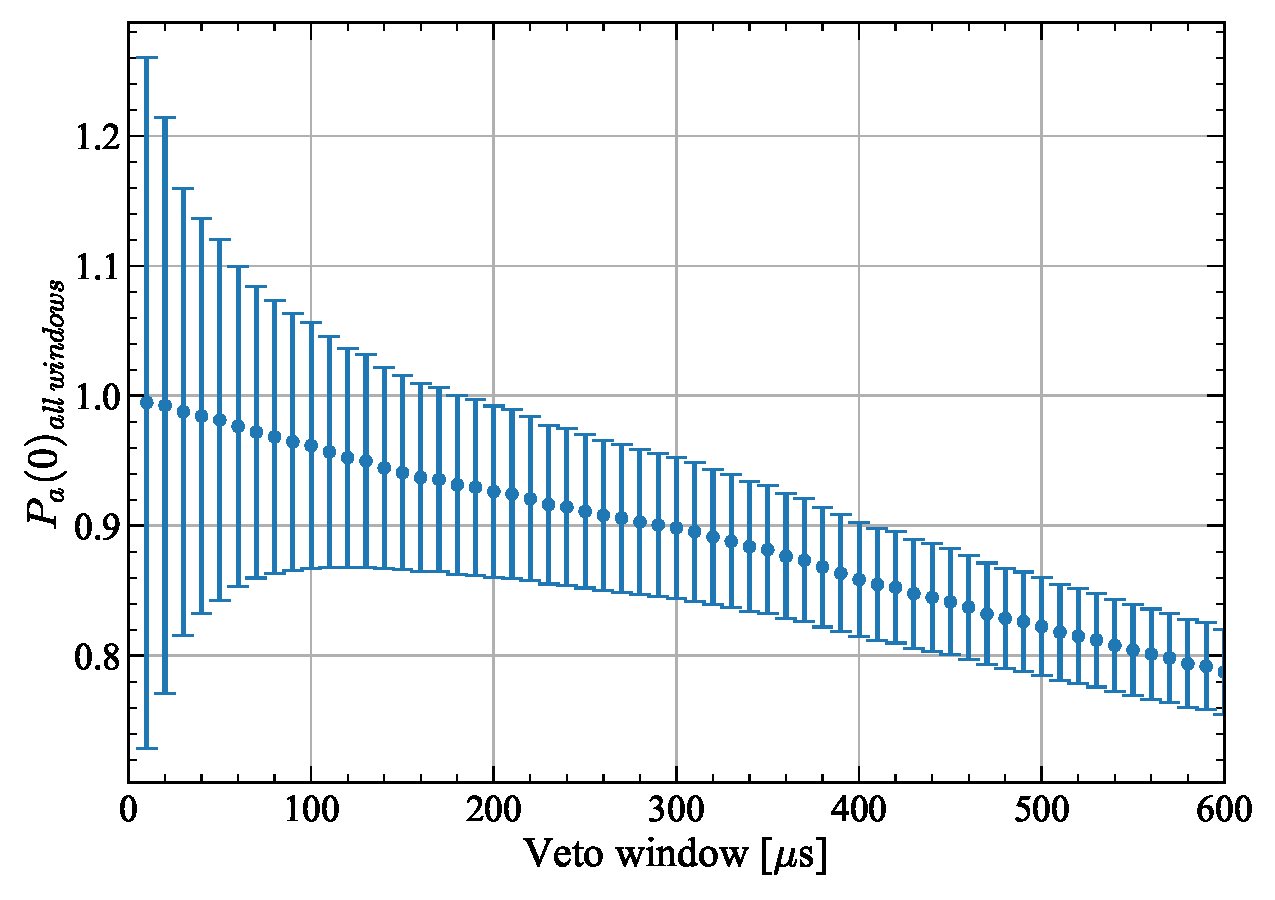
\includegraphics[width=\textwidth]{figures/VetoEfficiency/SR3AmLi_700mm_Corrections_100k.pdf}
        \caption{}
        \label{fig:VetoEff/SR3AmLi_700mm_Corrections}
    \end{subfigure}
    \hfill
    \begin{subfigure}[b]{0.49\textwidth}
        \centering
        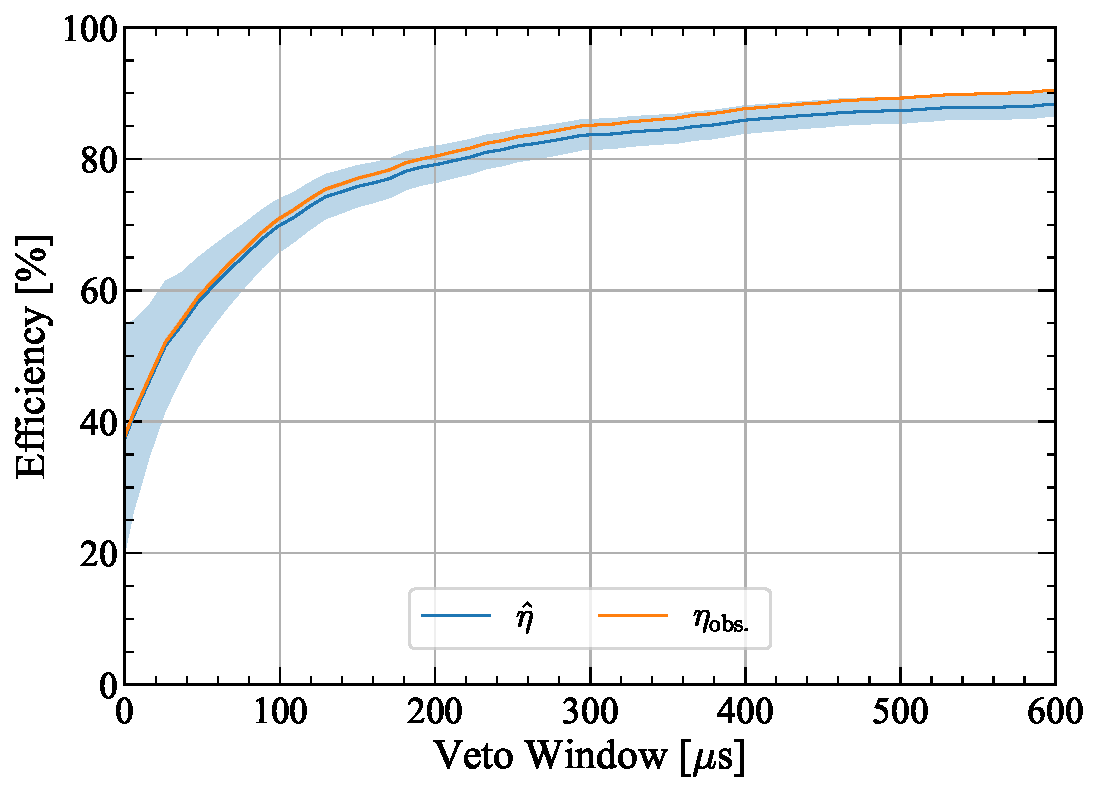
\includegraphics[width=\textwidth]{figures/VetoEfficiency/AmLiAccidentalCheck.pdf}
        \caption{}
        \label{fig:VetoEff/AmLiAccidentalCorrectionImpact}
    \end{subfigure}
    \caption{\textbf{Left:} $P_a(0)_{\text{all windows}}$ accidental correction factors over a 600~$\mu$s for AmLi calibration sources positioned at $z=700~\text{mm}$. The errors shown are only statistical uncertainties. \textbf{Right:} Comparison between calculated veto efficiencies for AmLi calibration sources positioned at $z=700~\text{mm}$ with accidental correction applied, $\eta_\text{true}$, and not applied, $\eta_\text{obs.}$.}
    \label{fig:VetoEff/AmLiAccidentalPlots}
\end{figure}

{\color{red}Few lines on efficiencies and ref the plots below.}
\begin{figure}[!ht]
    \centering
    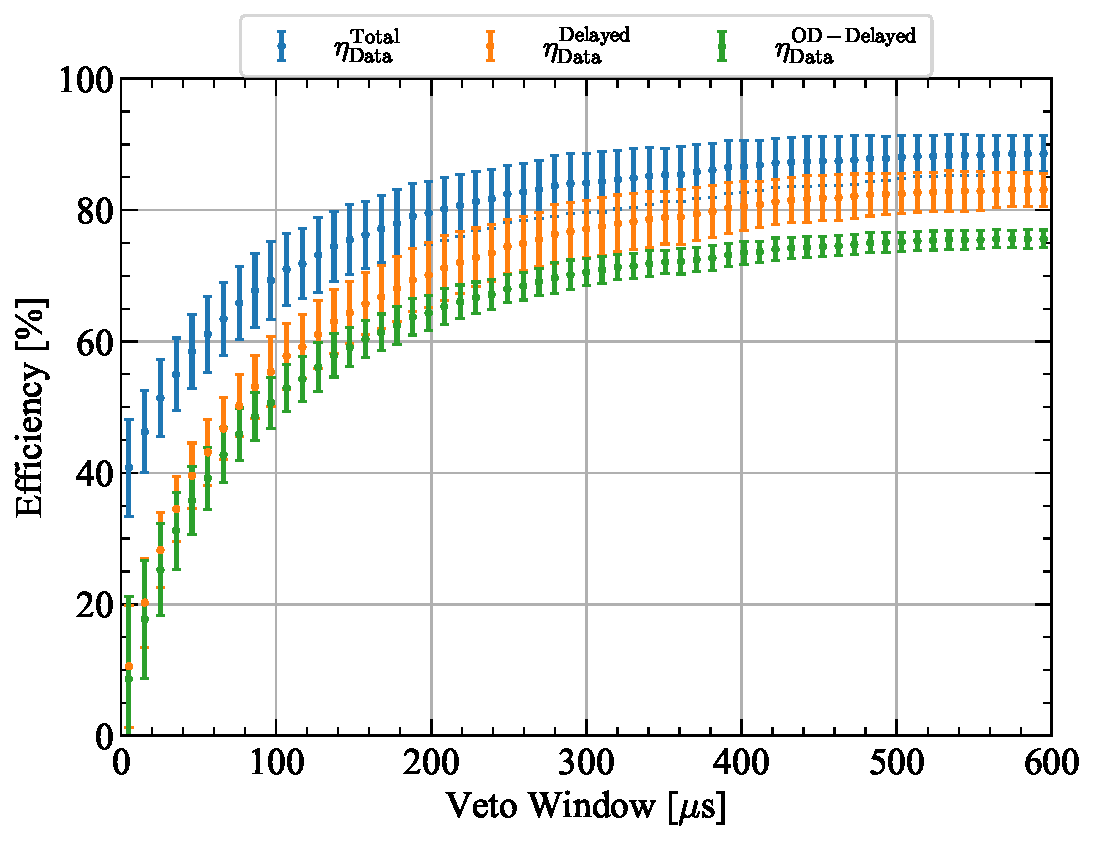
\includegraphics[width=0.7\textwidth]{figures/VetoEfficiency/AmLiEfficiencies_Data.pdf}
    \caption{AmLi Efficiencies}
    \label{fig:VetoEff/AmLiEfficiencies}
\end{figure}

\subsubsection{Deuterium-deuterium}
DD calibration data used in this study was taken during the October 2023 calibration campaign prior to the WS2024 science run. Events which were classified as single scatters by LZap and passed the selection outlined in \autoref{tab:VetoEff/dd_efficiency_cuts} were used for the study. In addition to these cuts an NR band selection, defined by \autoref{eqn:VetoEff/NRBandSelection}, is applied. It is important to note that DD NR band is different to AmLi NR band. The two different NR bands for the calibration sources is shown in \autoref{fig:VetoEff/SR3NRBands}.

\begin{table}[!ht]
	\centering
	\caption{Outline of cuts applied to DD calibration data for determining the veto efficiency. All cuts are defined in \autoref{tab:App_VetoEff/CoreCuts}.}
	\begin{tabular}{lll}
    \hline\hline
	\textbf{Physics cuts}&\textbf{S2 cuts}&\textbf{S1 cuts} \\
	\hline
	Single scatter & S2 width vs drift time & S1 prominence cut \\
	S1 and S2 threshold & Narrow S2 & Stinger event cut \\
	Fiducial Volume & S2 rise time & S1 TBA vs drift time \\
	& S2 early peak & S1 HSC cut \\
	& S2 XY quality & S1 shape \\
	& S2 TBA (above-anode gas) & S1 photon timing \\
    \hline\hline
	\end{tabular}
	\label{tab:VetoEff/dd_efficiency_cuts}
\end{table}
The DD calibration data is also corrected for accidental coincidences. The same method is used which is discussed in \autoref{sec:VetoEff/AmLiAccCorrection}. The correction factors used as a function of veto window is shown in \autoref{fig:VetoEff/DDAccCorrectionParameters}. At $600~\mu\text{s}$, $P_a(0)_{\text{all windows}}=0.88\pm0.11$. The impact of accidental coincidences on DD data is significantly less than AmLi as events are selected using the trigger from the DD neutron generator. The LZ DAQ is triggered by the generator during neutron production as neutrons are pulsed. The selection of events based on the generator trigger suppresses accidental coincidences. The impact of the accidental corrections on the observed DD veto efficiency is shown in \autoref{fig:VetoEff/DDAccCorrectionImpact_P0}.
\begin{figure}[!ht]
    \centering
    \begin{subfigure}[b]{0.49\textwidth}
        \centering
        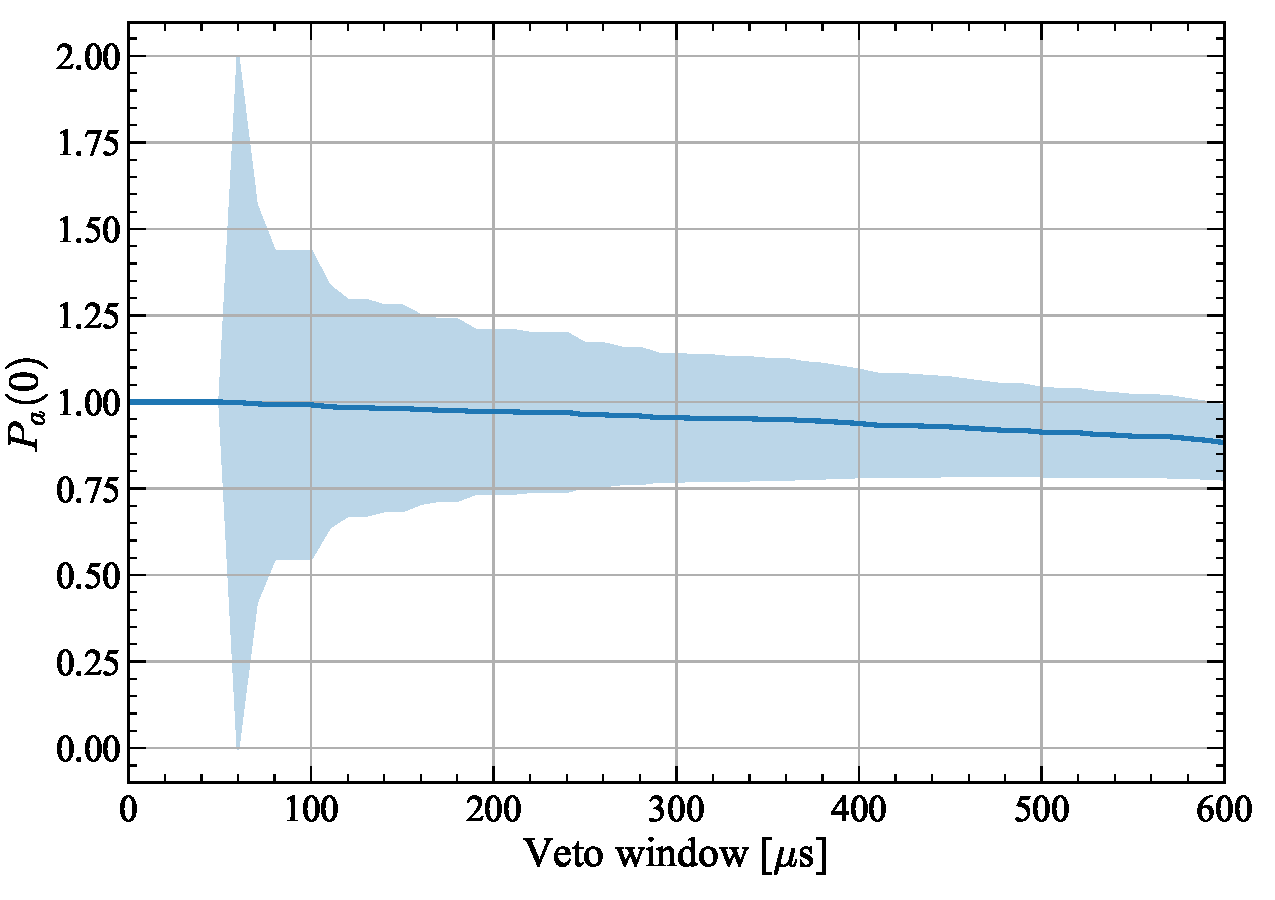
\includegraphics[width=\textwidth]{figures/VetoEfficiency/SR3DDdirect_Corrections_100k.pdf}
        \caption{}
        \label{fig:VetoEff/DDAccCorrectionParameters}
    \end{subfigure}
    \hfill
    \begin{subfigure}[b]{0.49\textwidth}
        \centering
        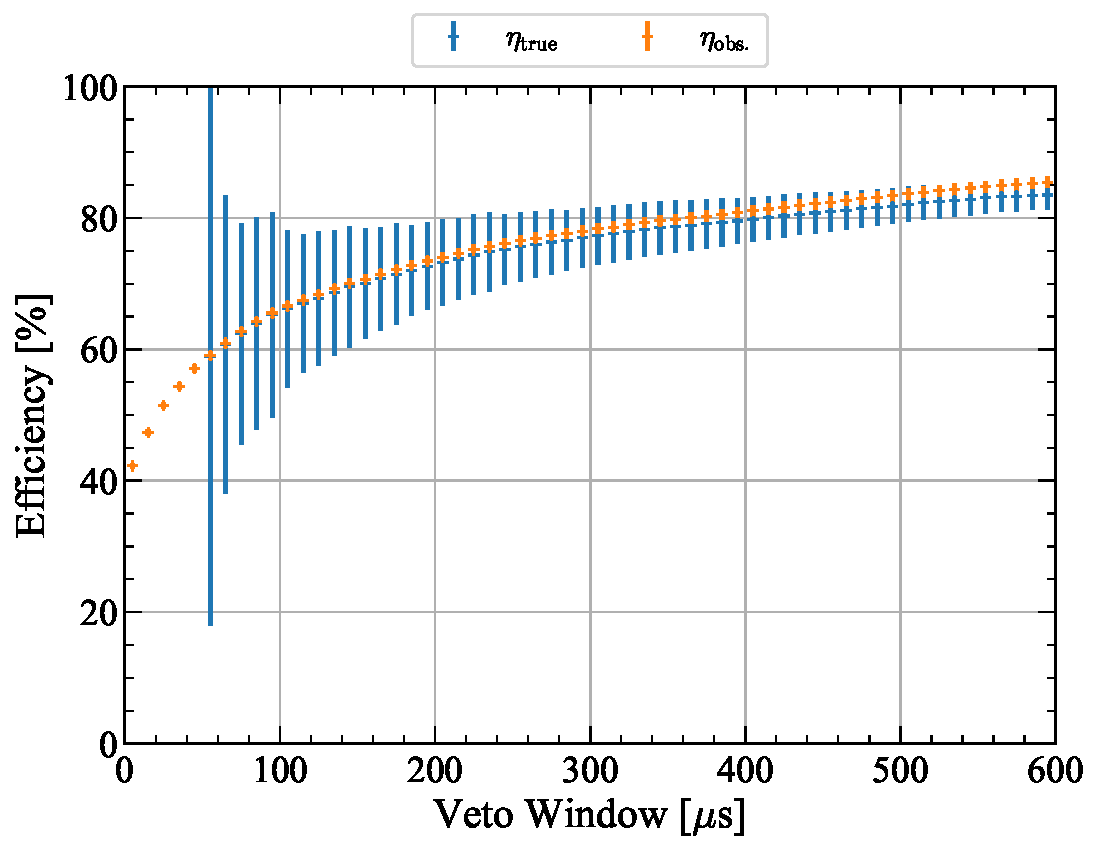
\includegraphics[width=\textwidth]{figures/VetoEfficiency/DDAccidentalCheck.pdf}
        \caption{}
        \label{fig:VetoEff/DDAccCorrectionImpact_P0}
    \end{subfigure}
    \caption{\textbf{Left:} $P_a(0)_{\text{all windows}}$ accidental correction factors over a 600~$\mu$s veto window for the DD calibration source data. The errors shown are only statistical uncertainties. \textbf{Right:} Comparison between calculated veto efficiencies for the DD calibration source with accidental correction applied, $\eta_\text{true}$, and not applied, $\eta_\text{obs.}$.}
    \label{fig:VetoEff/DDAccidentalPlots}
\end{figure}

{\color{red}Few lines on efficiencies and ref the plots below.}

\begin{figure}[!ht]
    \centering
    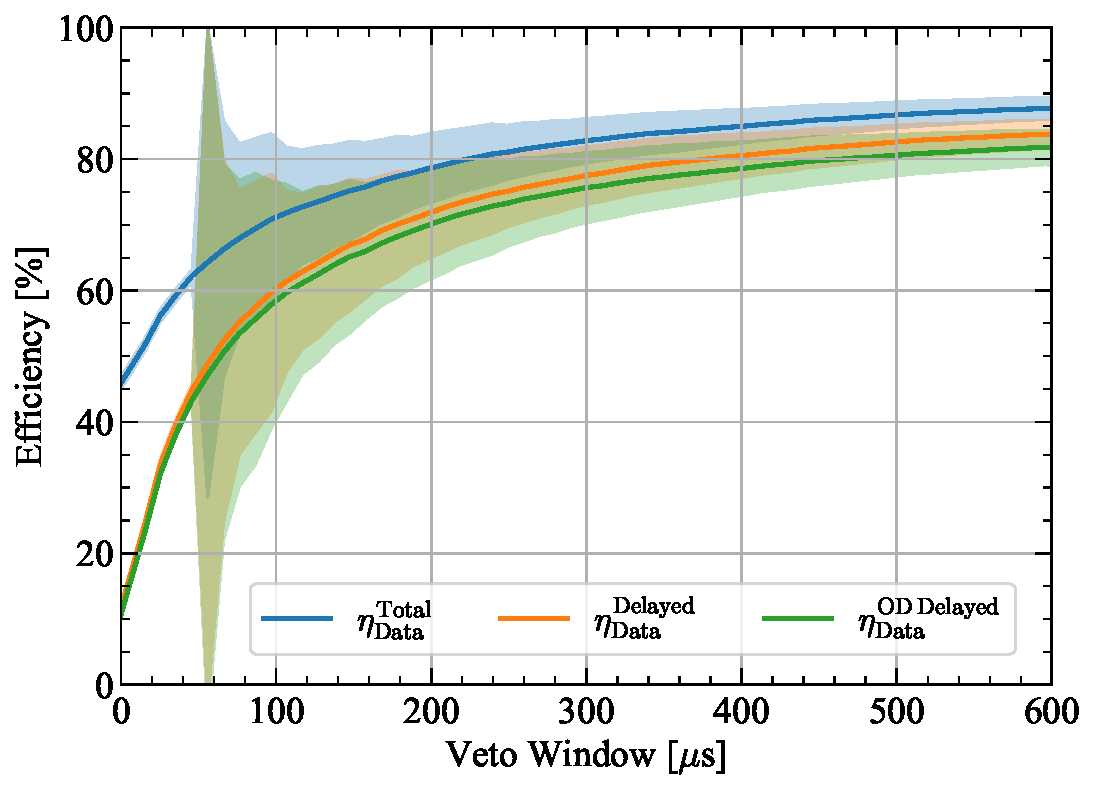
\includegraphics[width=0.7\textwidth]{figures/VetoEfficiency/DDEfficiencies_Data.pdf}
    \caption{DD Efficiencies}
    \label{fig:VetoEff/DDEfficiencies}
\end{figure}

\subsection{Simulated neutrons from calibration sources}
AmLi and DD calibration sources are simulated using LZ's \textit{fast} chain simulation technique (discussed in \autoref{sec:LZ/Simulations}). Simulated events which were classified as single scatters by LZLAMA and passed the selection outlined in \autoref{tab:VetoEff/calibration_simulation_efficiency_cuts} were used to determine the calculated veto efficiency.
As no accidental gammas or neutrons are present in the simulation, no accidental correction is needed.
{\color{red}Few lines on efficiencies and ref the plots below.}
\begin{figure}[!ht]
    \centering
    \begin{subfigure}[b]{0.49\textwidth}
        \centering
        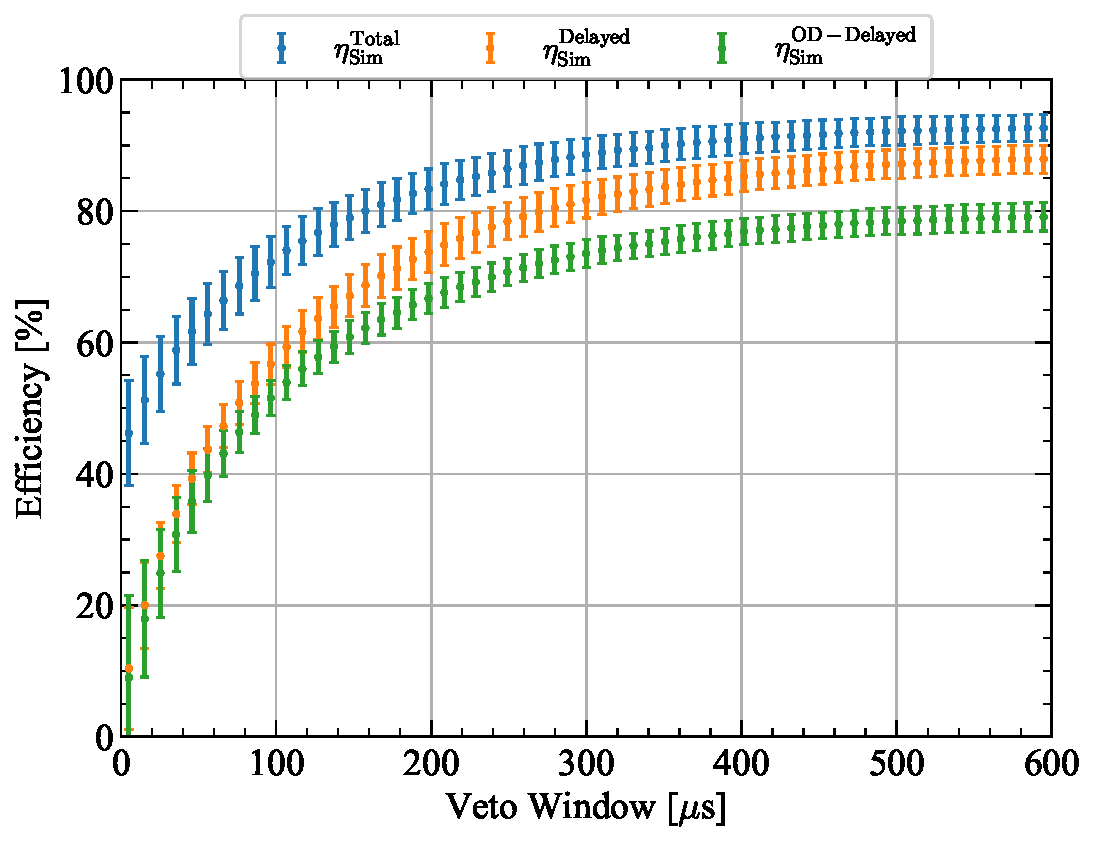
\includegraphics[width=\textwidth]{figures/VetoEfficiency/AmLiEfficiencies_Sim.pdf}
        \caption{}
        \label{fig:VetoEff/AmLiSimEfficiencies}
    \end{subfigure}
    \hfill
    \begin{subfigure}[b]{0.49\textwidth}
        \centering
        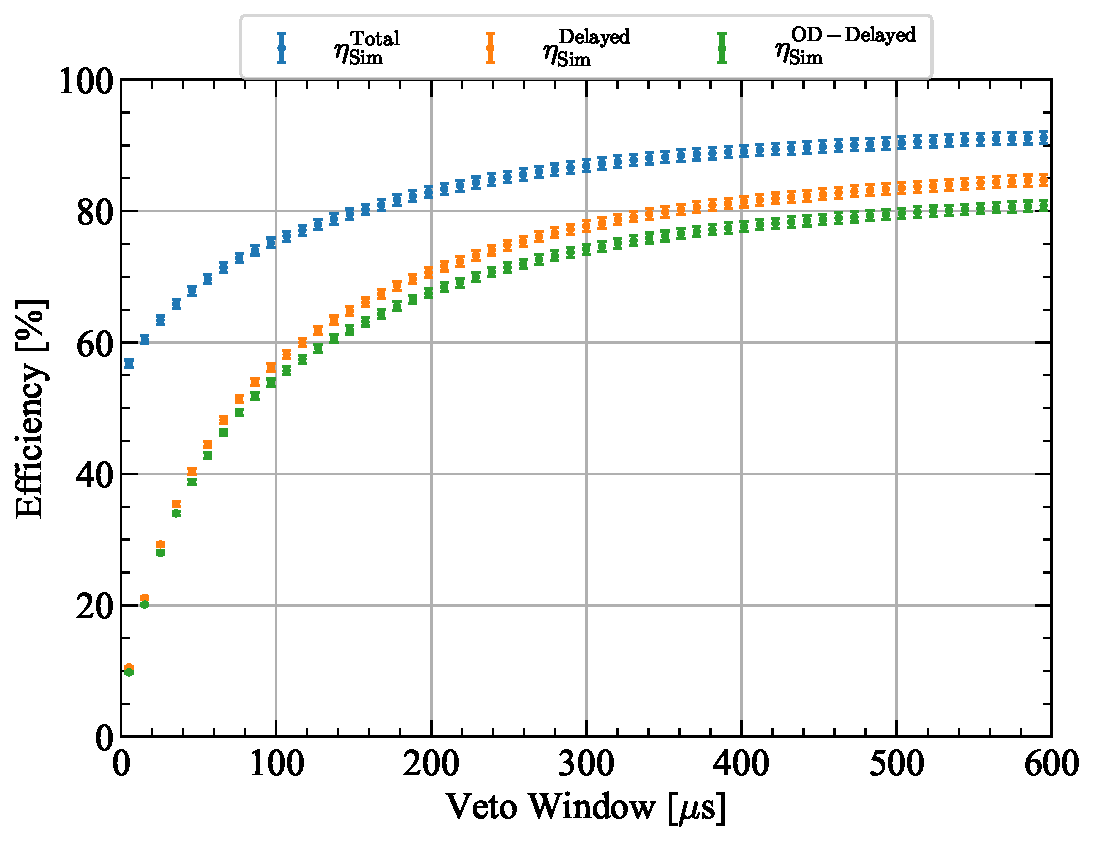
\includegraphics[width=\textwidth]{figures/VetoEfficiency/DDEfficiencies_Sim.pdf}
        \caption{}
        \label{fig:VetoEff/DDSimEfficiencies}
    \end{subfigure}
    \caption{Efficiencies...}
    \label{fig:VetoEff/Sim2DataVetoEffComparisons}
\end{figure}

The comparison between veto efficiencies calculated for data and simulation for both sources is shown in \autoref{fig:VetoEff/Sim2DataVetoEffComparisons}. The veto efficiency for AmLi is averaged across all CSD positions and $z$-positions. The percentage difference between the calculated veto efficiency is presented below the veto efficiency curves for both sources. Both sources show good agreement when total veto efficiencies are compared with $4.37\%$ and $2.39\%$ difference between data and simulation for AmLi and DD calibration sources respectively.
\begin{table}[!ht]
	\centering
	\caption{Outline of cuts applied to simulation data for determining the veto efficiency. All cuts are defined in \autoref{tab:App_VetoEff/CoreCuts} unless stated otherwise.}
	\begin{tabular}{l}
        \hline\hline
        \textbf{Physics cuts}\\
        \hline
        Single scatter\\
        S1 and S2 threshold\\
        Fiducial Volume\\
        CSD Selection (AmLi only, defined in \autoref{eqn:VetoEff/CSDSelection})\\
        NR Band Selection (defined in \autoref{eqn:VetoEff/NRBandSelection})\\
        \hline\hline
	\end{tabular}
	\label{tab:VetoEff/calibration_simulation_efficiency_cuts}
\end{table}

\begin{figure}[!ht]
    \centering
    \begin{subfigure}[b]{0.49\textwidth}
        \centering
        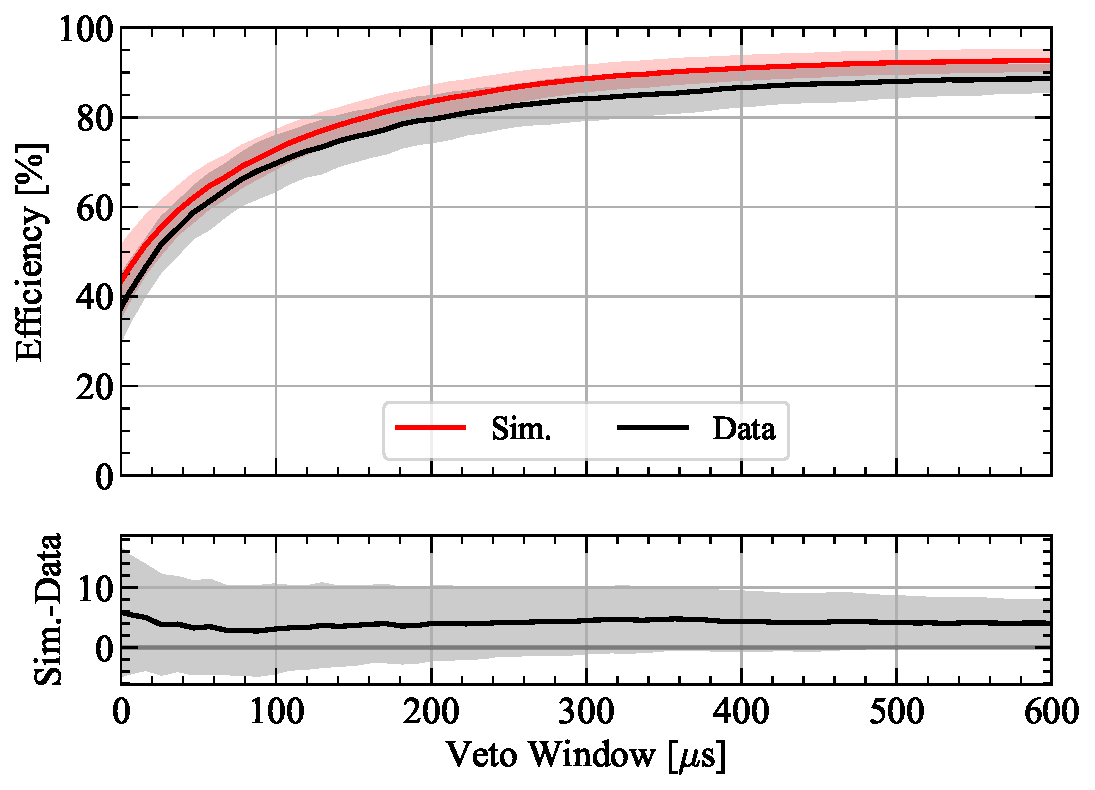
\includegraphics[width=\textwidth]{figures/VetoEfficiency/AmLi_Total_Avg_Ratio.pdf}
        \caption{}
        \label{fig:VetoEff/Sim2DataVetoEffComparisons_AmLi}
    \end{subfigure}
    \hfill
    \begin{subfigure}[b]{0.49\textwidth}
        \centering
        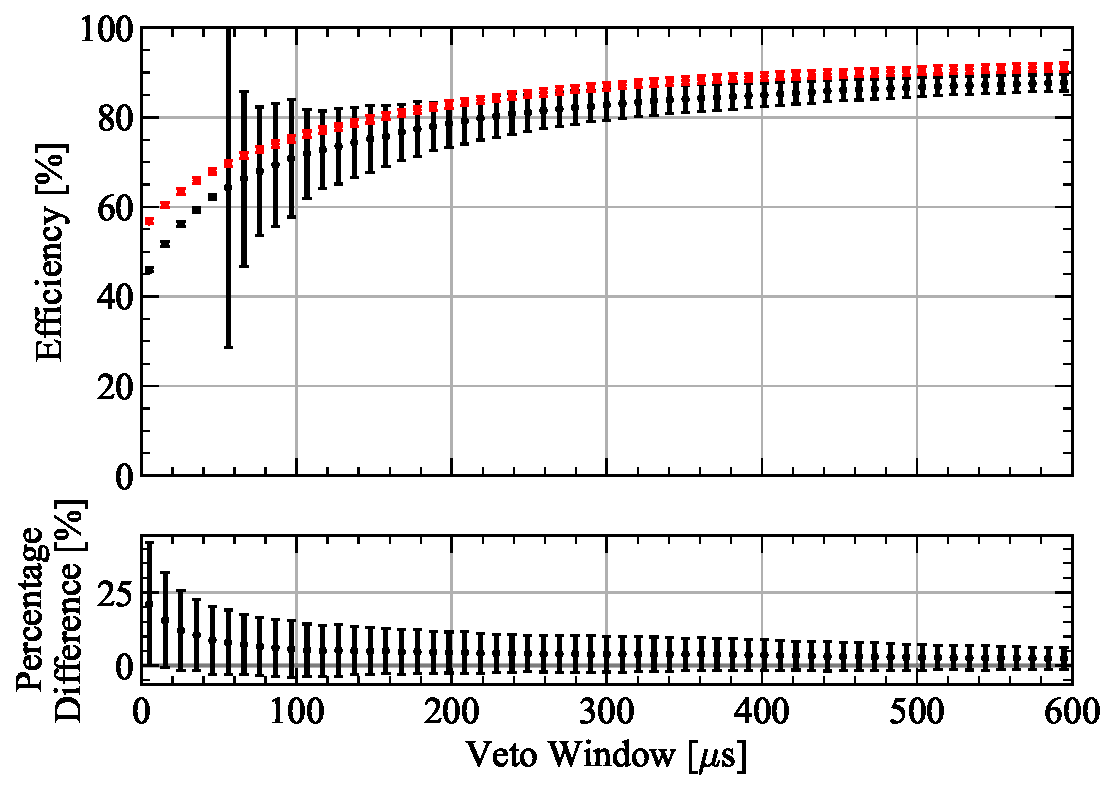
\includegraphics[width=\textwidth]{figures/VetoEfficiency/DDDirect_Total_Ratio.pdf}
        \caption{}
        \label{fig:VetoEff/Sim2DataVetoEffComparisons_DD}
    \end{subfigure}
    \caption{Comparison of calculated data (black) and simulation (red) veto efficiencies for AmLi (left) and DD (right) calibration sources. The percentage difference between the calculated veto efficiency is presented below the veto efficiency curves for both sources. Both sources show good agreement when veto efficiencies are compared with $4.37\%$ and $2.39\%$ difference between data and simulation for AmLi and DD calibration sources respectively.}
    \label{fig:VetoEff/Sim2DataVetoEffComparisons}
\end{figure}

\subsection{Background neutrons}
Detector NR simulations are produced using LZ's \textit{fast} chain simulation technique as part of the official LZ production prior to the WS2024 science run.
As part of this production each of the 644 components which have a radioactive background are simulated.
Simulated events which were classified as single scatters by LZLAMA and passed the selection outlined in \autoref{tab:VetoEff/detector_nr_simulation_efficiency_cuts} were used to determine the calculated veto efficiency.
The efficiency of tagging neutrons from Uranium Spontaneous Fission (USF) and ($\alpha$,n) events are shown in \autoref{fig:VetoEff/detector_nr_efficiency}. Also shown is the total efficiency.

\begin{table}[!ht]
	\centering
	\caption{Outline of cuts applied to detector NR simulations for determining the veto efficiency. All cuts are defined in \autoref{tab:App_VetoEff/CoreCuts}.}
	\begin{tabular}{l}
    \hline\hline
		\textbf{Physics cuts}\\
		\hline
		Single scatter\\
		S1 and S2 threshold\\
		Fiducial Volume\\
        \hline\hline
	\end{tabular}
	\label{tab:VetoEff/detector_nr_simulation_efficiency_cuts}
\end{table}

\begin{figure}[!ht]
	\centering
	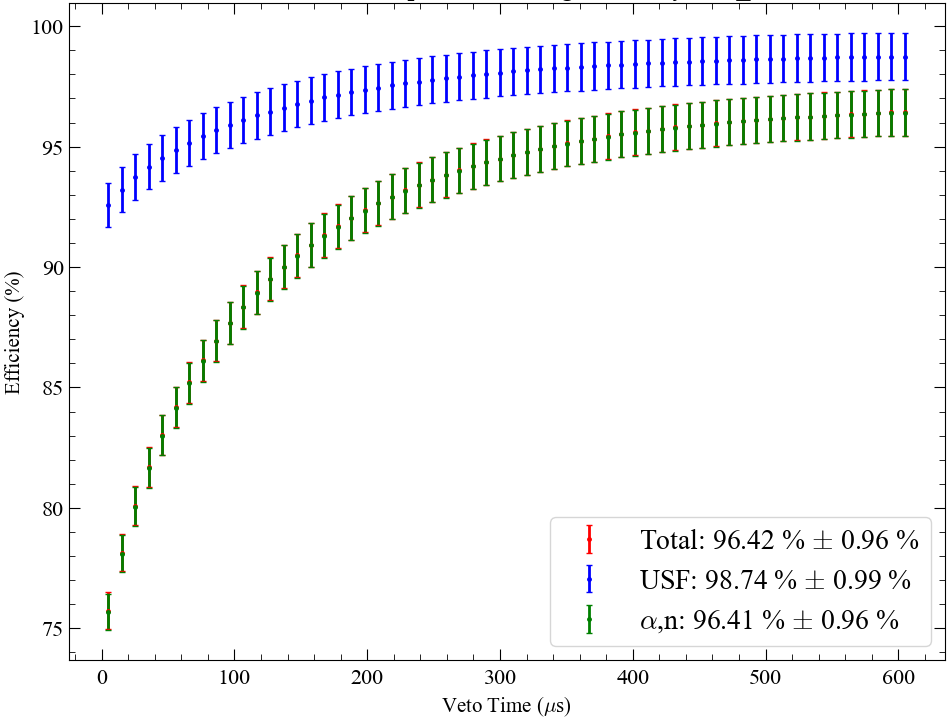
\includegraphics[width=0.7\textwidth]{figures/VetoEfficiency/det_nr_efficiency.png}
	\caption{Efficiency for tagging a neutron on detector NR simulations.}
	\label{fig:VetoEff/detector_nr_efficiency}
\end{figure}

\subsection{Background neutron efficiency from data}\label{sec:VetoEff/BkgNeutronEff}
The neutron veto efficiency from each calibration source from data and simulation is shown in \autoref{fig:VetoEff/efficiency_summary}. Also shown is the efficiency from simulated background neutrons.
The $z$-position of each point is calculated from the mean drift time, $\overline{t}_{\text{drift}}$, of events which pass the selection outlined in \autoref{tab:VetoEff/detector_nr_simulation_efficiency_cuts}.
For the detector NR simulations, the events were split up into three $z$-sections by the following:
\begin{itemize}
    \item \textit{Top: } $71~\mu \text{s}<\overline{t}_{\text{drift}}\leq350~\mu \text{s}$
    \item \textit{Middle: } $350~\mu \text{s}<\overline{t}_{\text{drift}}\leq700~\mu \text{s}$
    \item \textit{Bottom: } $700~\mu \text{s}<\overline{t}_{\text{drift}}\leq1030~\mu \text{s}$
\end{itemize}

\begin{figure}[!ht]
	\centering
	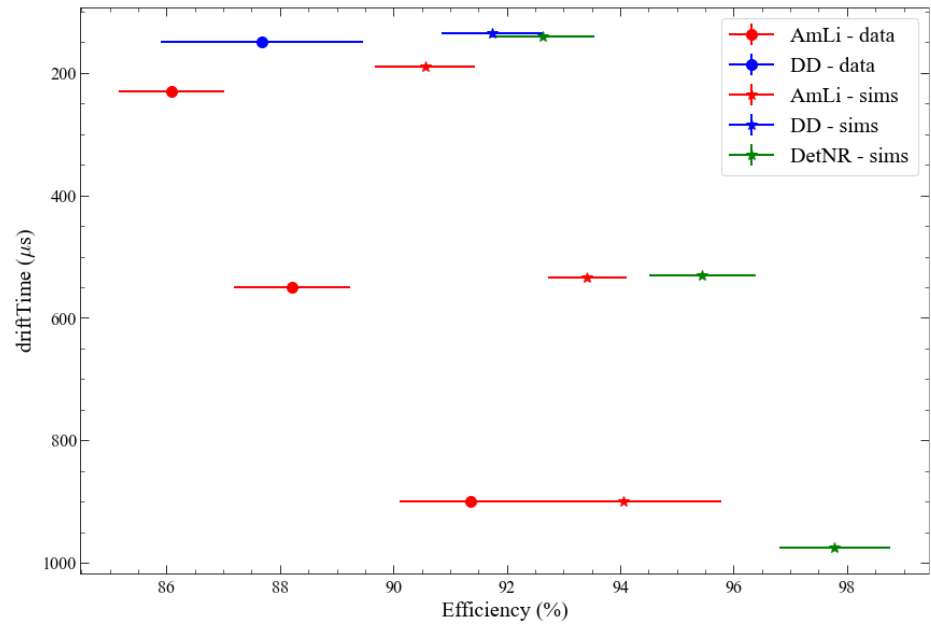
\includegraphics[width=0.7\textwidth]{figures/VetoEfficiency/efficiency_summary.png}
	\caption{Summary of efficiency from all simulations and calibration sources.
		The CSD sources are averaged at each deployment position, $z=100~\text{mm},700~\text{mm},1300~\text{mm}$.
		Circle markers represent calculated veto efficiencies from data.
		Star markers represent calculated veto efficiencies from simulation.}
	\label{fig:VetoEff/efficiency_summary}
\end{figure}
This $t_{\text{drift}}$ splitting of detector NR simulation is performed to compare the calculated veto efficiencies of the detector NR simulations to veto efficiencies calculated from calibration sources. However, this was not used in the final efficiency evaluation. Shown in \autoref{tab:VetoEff/final_veto_efficiency} are the veto efficiencies of all calibration sources for both simulations and data alongside the veto efficiencies for the detector NR sources.

The importance of this chapter lies in determining LZ's efficiency to reject background neutrons, the estimated veto efficiency for detector NR events, $\eta_{\text{Det. NR}}^{\text{Data}}$. The method to estimate this efficiency is as follows. 
The average simulation calibration efficiency is taken between, $\overline{\eta}_{\text{AmLi}}^{\text{Sim.}}=(92.8\pm2.0)\%$ and $\eta_{\text{DD}}^{\text{Sim.}}=(91.8\pm1.0)\%$ which results in an average efficiency of $\overline{\eta}_{\text{Cal.}}^{\text{Sim.}}=(92.3\pm1.1)\%$.
The average data calibration efficiency is taken between, $\overline{\eta}_{\text{AmLi}}^{\text{Data}}=(88.6\pm2.7)\%$ and $\eta_{\text{DD}}^{\text{Data}}=(91.8\pm1.0)\%$, which results in an average efficiency of $\overline{\eta}_{\text{Cal.}}^{\text{Data}}=(88.2\pm1.6)\%$.
The difference, $\Lambda$, between the simulation calibration and data calibration efficiencies is then used as a systematic uncertainty on the efficiency of detector NR simulations.
This process is expressed in \autoref{eqn:VetoEff/DetNR_efficiency}, and gives an estimated veto efficiency for detector NR of $\eta_{\text{Det. NR}}^\text{Data}=(92.2\pm4.3)\%$.
The final uncertainty of the estimated detector NR veto efficiency, $\sigma^\text{Data}_\text{Det. NR}$, is the product of the statistical uncertainty from the simulations $\sigma^\text{Sim.}_\text{Det. NR}=1\%$, and $\Delta=4.2\%$ from the subtraction of the data calibration efficiency from the simulation calibration efficiency.
\begin{equation}
    \label{eqn:VetoEff/DetNR_efficiency}
    \begin{split}
    	\overline{\eta}_{\text{Cal.}}^{\text{Sim.}} & = \frac{\overline{\eta}_{\text{AmLi}}^{\text{Sim.}}+\eta_{\text{DD}}^{\text{Sim.}}}{2}\\
    	\overline{\eta}_{\text{Cal.}}^{\text{Data}} & = \frac{\overline{\eta}_{\text{AmLi}}^{\text{Data}}+\eta_{\text{DD}}^{\text{Data}}}{2} \\
    	\Lambda &= \overline{\eta}_{\text{Cal.}}^{\text{Sim.}} - \overline{\eta}_{\text{Cal.}}^{\text{Data}}\\
    	\eta_\text{Det. NR}^\text{Data}   & = \eta_\text{Det. NR}^\text{Sim.} - \Lambda
    \end{split}
\end{equation}
For the 2024 WIMP search result \cite{LZ:2024zvo}, LZ achieved an estimated neutron tagging efficiency, $\eta_\text{Det. NR}^\text{Data}=(92\pm4)\%$.

\begin{table}[!ht]
	\centering
	\caption[Summary of veto tagging efficiencies.]{Summary of veto tagging efficiencies.}
	\begin{tabular}{lll}
    \hline\hline
    \textbf{Source}& \textbf{$\eta^\text{Sim.}$}& \textbf{$\eta^\text{Data}$}\\ 
    \hline
    AmLi (average) & (92.8$\pm$2.0)\% & (88.6$\pm$2.7)\% \\
    DD (Direct)    & (91.8$\pm$1.0)\% & (87.7$\pm$1.8)\% \\
    Detector NR    & (96.4$\pm$1.0)\% & (92.2$\pm$4.3)\%\\
    \hline\hline
	\end{tabular}
	\label{tab:VetoEff/final_veto_efficiency}
\end{table}


\section{Veto efficiency and the WIMP search}\label{sec:VetoEff4WIMPSearch}
\textcolor{red}{ToDo Need to talk about how the neutron efficiency is used in the WS result?}

\section{Concluding remarks}